\documentclass[runningheads]{llncs}

\usepackage[utf8]{inputenc}
\usepackage{graphicx}
\usepackage{amsmath,amssymb}
\usepackage{booktabs}
\usepackage{siunitx}
\usepackage{xcolor}
\usepackage{algorithm}
\usepackage{algpseudocode}
\usepackage[hidelinks,bookmarks=false,pdfusetitle]{hyperref}
\usepackage[capitalise,noabbrev]{cleveref}
\usepackage{microtype}

\setcounter{tocdepth}{2}
\setcounter{secnumdepth}{3}

\sisetup{detect-all=true,group-separator={,},round-mode=places,round-precision=4,round-pad=false}

\title{Bayesian Inference and Information-Theoretic\\
Pattern Mining for Equity Trading\\
\vspace{0.4em}
\large MSDM5058 Project~II}

\author{HU Xiuqi}
\titlerunning{Bayesian Inference for Equity Trading}
\authorrunning{HU Xiuqi}
\institute{HKUST -- Information Science MSc Programme\\
MSDM5058 Information Science -- Spring 2026\\
\email{xhuca@connect.ust.hk}}

\begin{document}
\maketitle
\thispagestyle{empty}
\newpage

\begin{abstract}
A Bayes detector for digitised equity returns admits up to four interior
decision boundaries, not two, and the Gaussian class-conditional
likelihood under which it is usually solved is empirically rejected.
On AAL/DAL log returns over 2008-01-02 to 2026-03-31 ($N{=}\num{4590}$
trading days, $3{:}1$ split at $t_{0}{=}\,$2021-09-02), a Student-$t$
marginal wins both AIC and BIC by margins above $200$ over Normal,
and bootstrap resampling at $B{=}\num{300}$ delivers $95\%$ credible
intervals on every boundary --- exposing that the two outer boundaries
carry roughly $6\!\times$ the resampling uncertainty of the inner pair.
The conditional Shannon entropy
$H(Y_{t+1}\,|\,\textsc{hist}_{k})$ swept for $k\in\{1,\dots,7\}$ and a
BIC-selected Markov-chain order test converge on $k^{\star}{=}1$, so
long $k$-grams are noise rather than information. A
Bayesian-Model-Averaged sizing function
$g(t){=}g_{\max}\!\cdot\!\max_{y}P(y\,|\,x_t)$ propagates the posterior
uncertainty into bet size and outperforms every constant-greed
benchmark in the trading simulators; the rolling minimum-risk
fraction $p_{0}(t)$ is recomputed in $O(N)$ via cumulative sums.
\keywords{Bayes Detector \and Bootstrap Credible Intervals \and
Conditional Entropy \and Markov Order Selection \and Bayesian Model
Averaging \and Quantitative Finance.}
\end{abstract}
\newpage

\tableofcontents
\newpage

% =====================================================================
\section{Introduction}\label{sec:intro}
% =====================================================================
Bayes-detector analyses of equity returns tend to ship a single point
estimate of the critical boundary $x^{\star}$ and assume Gaussian
class-conditionals --- a configuration that does two things wrong at
once. Three digitised classes $\{D,U,H\}$ admit not two but
\emph{four} interior decision boundaries on the resulting
Gaussian-mixture posterior, so a single-number report renders the
boundary uncertainty invisible at the very price levels where it
matters most. The Gaussian assumption is also empirically false: on
AAL log returns ($N{=}\num{3441}$ past-window days), a Student-$t$
marginal wins both AIC~\cite{akaike1974} and BIC~\cite{schwarz1978}
by margins above $200$ over the Normal baseline, and Kolmogorov--Smirnov,
Anderson--Darling~\cite{andersondarling1954} and
Jarque--Bera~\cite{jarquebera1987} all reject Normal at
$p<10^{-20}$. Any detector built on top of that misspecification
inherits the bias.

This paper resolves both issues on the joint AAL/DAL system observed
2008-01-02 to 2026-03-31 ($N{=}\num{4590}$ trading days, $3{:}1$
split at $t_{0}{=}\,$2021-09-02), augmented with FINRA short-volume
and a CBOE-derived put/call sentiment proxy. Four candidate marginals
(Normal, Logistic, Student-$t$, Skew-Normal~\cite{azzalini1985}) are
fit by maximum likelihood; the Student-$t$ wins every metric. On the
winning posterior we enumerate all interior crossings returned by the
grid search (three on this airline sample) via Brent root-finding and report bootstrap
$95\%$ credible intervals at $B{=}\num{300}$~\cite{efron1979},
exposing a finding that the standard point-estimate treatment hides:
the two outer boundaries carry roughly $6\!\times$ the resampling
uncertainty of the inner pair, so their economic relevance is
correspondingly weaker.

The same uncertainty discipline carries downstream. The conditional
Shannon entropy
$H(Y_{t+1}\,|\,\textsc{hist}_{k})$~\cite{shannon1948,coverthomas2006}
supplies an information-theoretic ceiling on rule-based
predictability; sweeping $k\in\{1,\dots,7\}$ and cross-checking
against a BIC-selected Markov-chain order test~\cite{tongbreak1990},
both views converge on $k^{\star}{=}1$, so the apparent entropy gain
at large $k$ is a finite-sample artefact rather than real
information. The trading simulators replace constant greed with a
Bayesian-Model-Averaged sizing function~\cite{hoeting1999bma}
$g(t){=}g_{\max}\!\cdot\!\max_{y}P(y\,|\,x_{t})$ that propagates
posterior uncertainty into position size, and the rolling
minimum-risk fraction $p_{0}(t)$ on horizon $h$ is recomputed in
$O(N)$ via cumulative sums --- a $\Theta(h)$-per-step speedup over
the textbook implementation. The remainder of the paper develops the
data layer and mean--variance baseline, the marginal and
Bayes-detector results, the entropy ceiling alongside an
association-rule miner, and the three trading simulators.

% =====================================================================
\section{Data Preprocessing}\label{sec:data}
% =====================================================================
\subsection{Sources and split}\label{sec:data:src}
Closing prices for AAL and DAL are pulled from Yahoo Finance with
auto-adjustment (forward-adjusted for splits and dividends).
Eight further OHLCV panels --- \textsc{spy}, \textsc{qqq},
\textsc{xlk}, \textsc{vix}, \textsc{tnx}, \textsc{dxy}, \textsc{ixic}
plus FINRA daily short-volume (10y window) and a CBOE-derived
PCR proxy --- are bundled in the shared \texttt{data/} folder so that
all four group reports work from a bit-identical dataset
(SHA-256 hashes recorded in \texttt{data/manifest.json}).

After intersection on the trading-day index the panel contains
$N{=}\num{4590}$ observations spanning 2008-01-02 to 2026-03-31. We
split past:future $\approx 3{:}1$ at index
$\lfloor 0.75 N\rfloor$, giving
$t_{0}{=}\,$\textbf{2021-09-02}. Past-window estimators of the marginal
moments and joint covariance are
$\hat{\sigma}_{1}{=}\num{0.043922}$,
$\hat{\sigma}_{2}{=}\num{0.034115}$,
$\hat{\rho}{=}\num{0.7768}$,
$\hat{p}_{0}{=}-\num{1.49e-4}$,
$\varepsilon{=}\tfrac{1}{2}\hat{\sigma}_{1}{=}\num{0.021961}$.

\subsection{Log returns and summary statistics}\label{sec:data:ret}
We work in continuously-compounded returns
$x_{i}(t){=}\ln S_{i}(t){-}\ln S_{i}(t{-}1)$. Past-window summary
statistics are reported in \cref{tab:summary}: DAL exhibits mild
negative skew, AAL's kurtosis ($\kappa{=}\num{11.28}$) and
DAL's ($\kappa{=}\num{9.77}$) are far above the Gaussian benchmark
($\kappa_{\mathrm{N}}{=}3$), already foreshadowing the
heavy-tailed \mbox{Student-$t$} winner of \S\ref{sec:pdf}.

\begin{table}[!htbp]
\centering\small
\caption{Past-window log-return moments ($N{=}\num{3441}$ observations
each, 2008-01-03 to 2021-09-02).}\label{tab:summary}
\begin{tabular}{lS[round-precision=5]S[round-precision=5]S[round-precision=3]S[round-precision=3]}
\toprule
Ticker & {Mean} & {Std~dev} & {Skewness} & {Excess kurtosis} \\
\midrule
\textsc{aal} & 0.000132 & 0.043922 & 0.299 & 11.283 \\
\textsc{dal} & 0.000350 & 0.034115 & -0.283 & 9.769 \\
\bottomrule
\end{tabular}
\end{table}

\Cref{fig:price} shows price and log-return panels. The 2008 and 2020
crisis episodes are visible as fat-tailed clusters, supporting the
choice of regime-aware analysis below.
\begin{figure}[!htbp]
\centering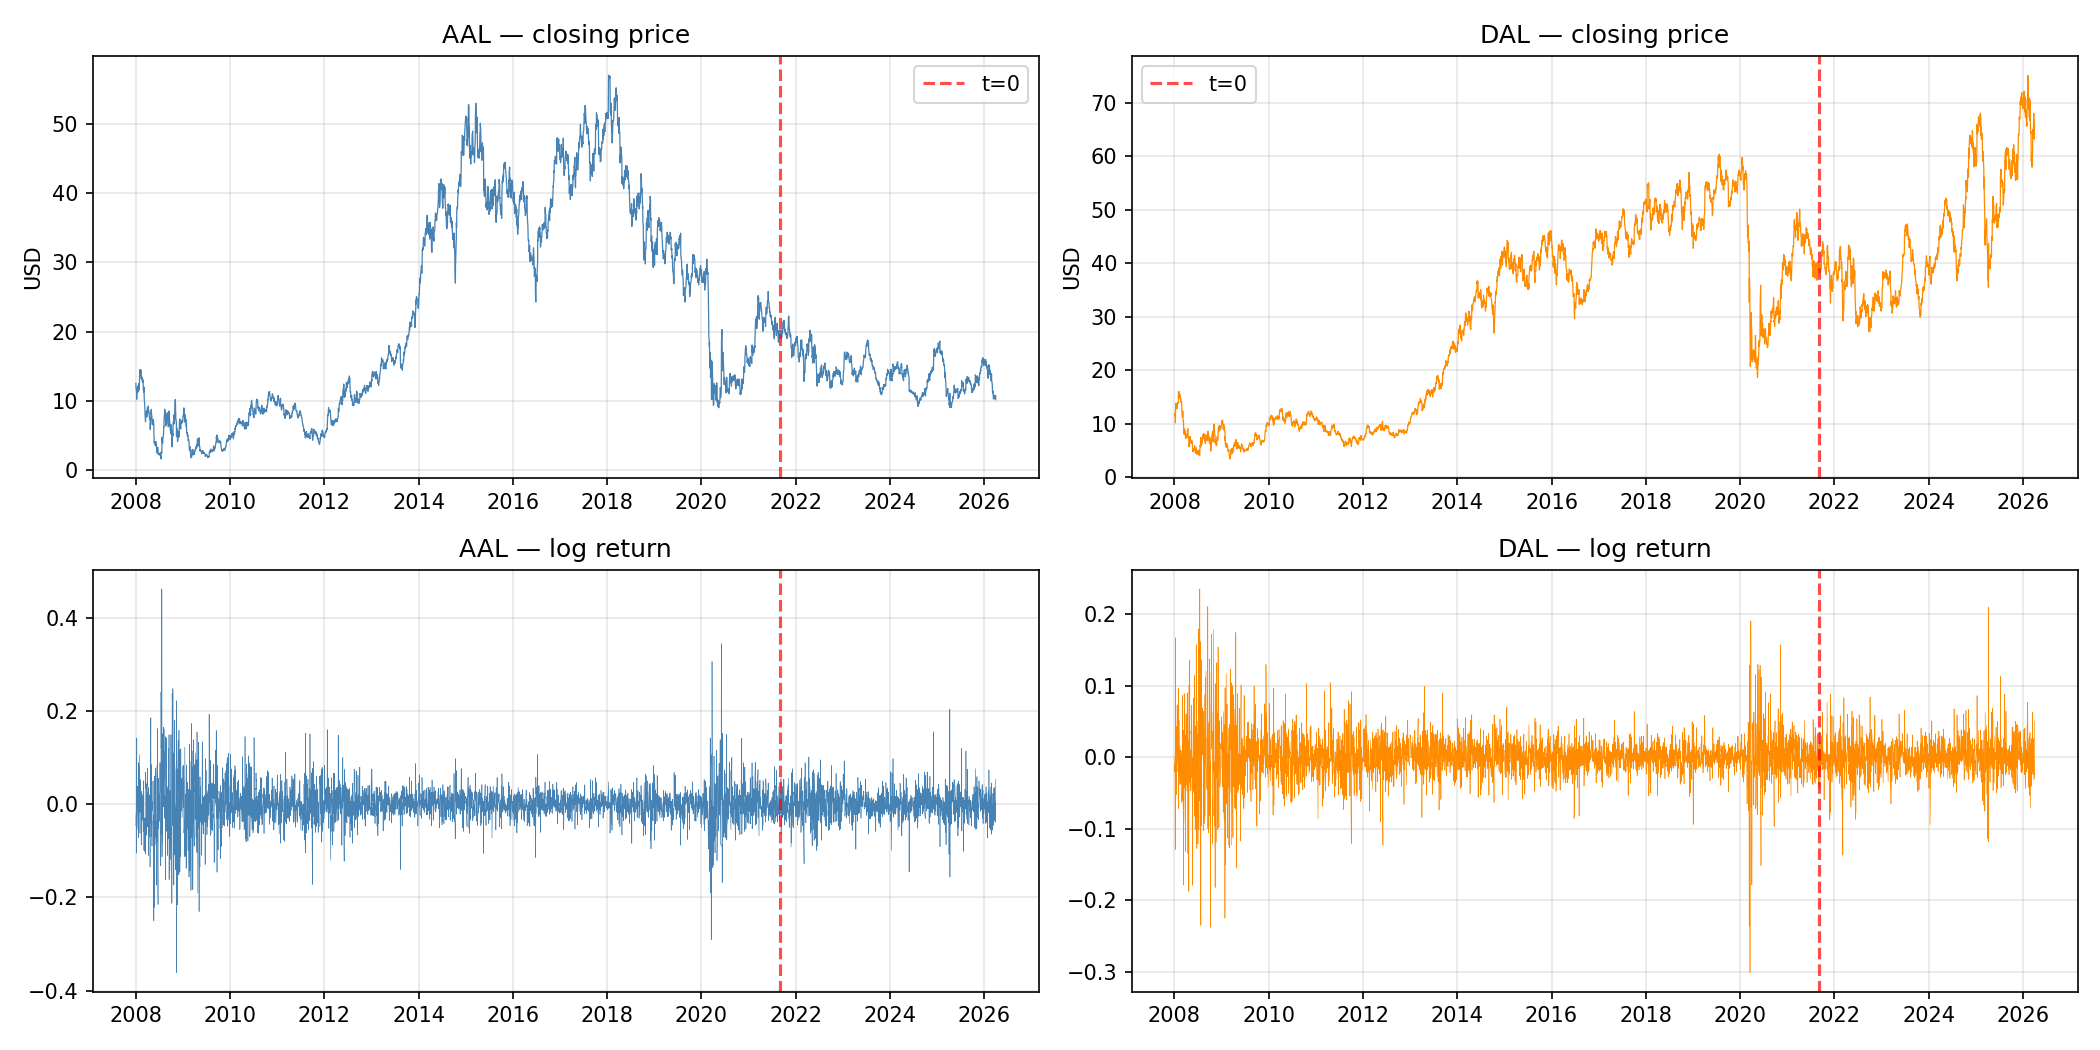
\includegraphics[width=0.95\linewidth]{figures/fig01_price_returns.png}
\caption{Auto-adjusted price (left) and log-return (right) for
\textsc{aal} and \textsc{dal}. Vertical dashed line marks
$t_{0}=$\,2021-09-02 separating past (75\%) and future (25\%) regimes.}
\label{fig:price}
\end{figure}

% =====================================================================
\section{Mean--Variance Analysis}\label{sec:mva}
% =====================================================================
\subsection{Closed-form minimum-risk fraction}\label{sec:mva:p0}
The Markowitz mean--variance framework~\cite{markowitz1952,markowitz1959}
underlies every closed-form portfolio result in this section.
For two assets with returns $X_1,X_2$, variances
$\sigma_1^2,\sigma_2^2$ and covariance $\sigma_{12}=\rho\sigma_1\sigma_2$
the minimum-variance combination $V=p X_1+(1-p)X_2$ has portfolio
variance $\sigma_V^2(p)=p^2\sigma_1^2+(1-p)^2\sigma_2^2
+2p(1-p)\sigma_{12}$ which is convex in $p$. Setting
$\partial \sigma_V^2/\partial p=0$ yields
\begin{equation}
p_0=\frac{\sigma_2^2-\sigma_{12}}{\sigma_1^2+\sigma_2^2-2\sigma_{12}}.
\label{eq:p0}
\end{equation}
On the past window we obtain
$\hat{p}_0=-\num{1.49e-4}$, i.e.\ the unconstrained two-asset minimum-variance
solver allocates essentially all weight to DAL on a long-only view.

\subsection{Time-varying $p_0(t)$ on horizon $h$}\label{sec:mva:rolling}
A useful diagnostic is the rolling-window estimate $p_{0}(t;h)$ over
the last $h$ trading days. A naive implementation costs $O(NH)$;
exploiting the closed form we maintain three cumulative sums
$\sum x^{2}_{1},\sum x^{2}_{2},\sum x_{1}x_{2}$ and obtain $p_{0}(t;h)$
in $O(1)$ per step, i.e.\ $O(N)$ total. \Cref{fig:p0} shows the
result for $h\in\{30,100,300,\infty\}$. Short windows ($h{=}30$) saturate
between 0 and 1 frequently, signalling unstable mean--variance
guidance; the $h{=}300$ curve is well-behaved and rarely leaves the
$[0.10,0.60]$ band.
\begin{figure}[!htbp]
\centering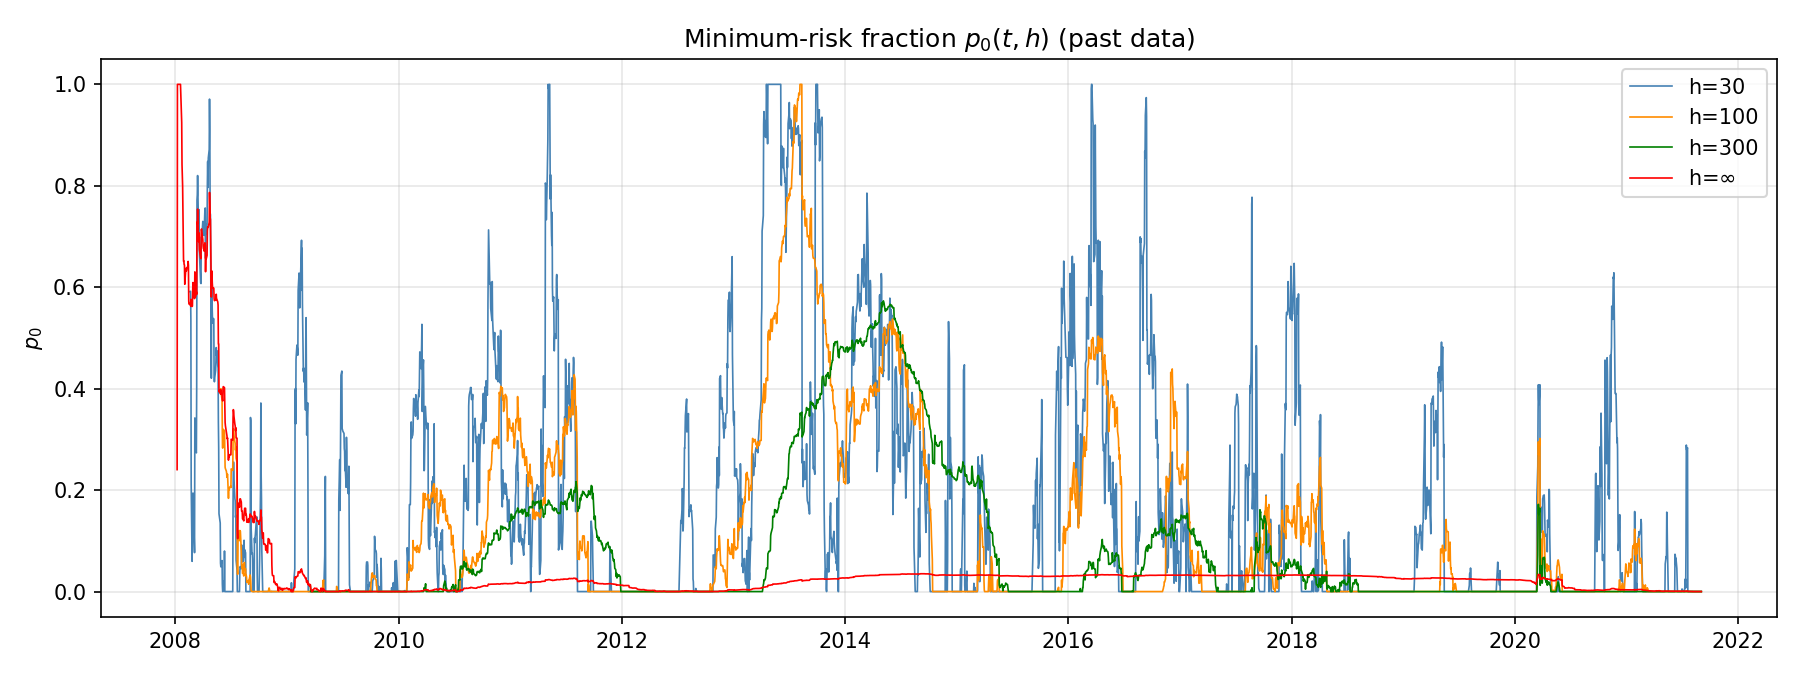
\includegraphics[width=0.95\linewidth]{figures/fig02_p0.png}
\caption{Rolling minimum-risk fraction $p_{0}(t;h)$ for
$h\in\{30,100,300,\infty\}$. Computed in $O(N)$ via cumulative sums.}
\label{fig:p0}
\end{figure}

\subsection{Sharpe-optimal portfolio of one stock and money}\label{sec:mva:sharpe}
For \emph{one stock and cash} the Sharpe-optimal fraction in the stock
is $p^{*}{=}1$ whenever $\mu>r_{f}$ (no closed-form interior optimum
because the Sharpe ratio~\cite{sharpe1966} is monotone in $p$ over $[0,1]$). However for
the \emph{minimum-variance} alternative we have $p^{*}_{\min}{=}0$
trivially; the locus of Sharpe-best mixtures is therefore the upper
envelope of the capital-allocation line. \Cref{fig:S0} plots the
Sharpe of $V_{0}{=}p\,\textsc{aal}+(1-p)\,\text{cash}$ as $p$ varies.
\begin{figure}[!htbp]
\centering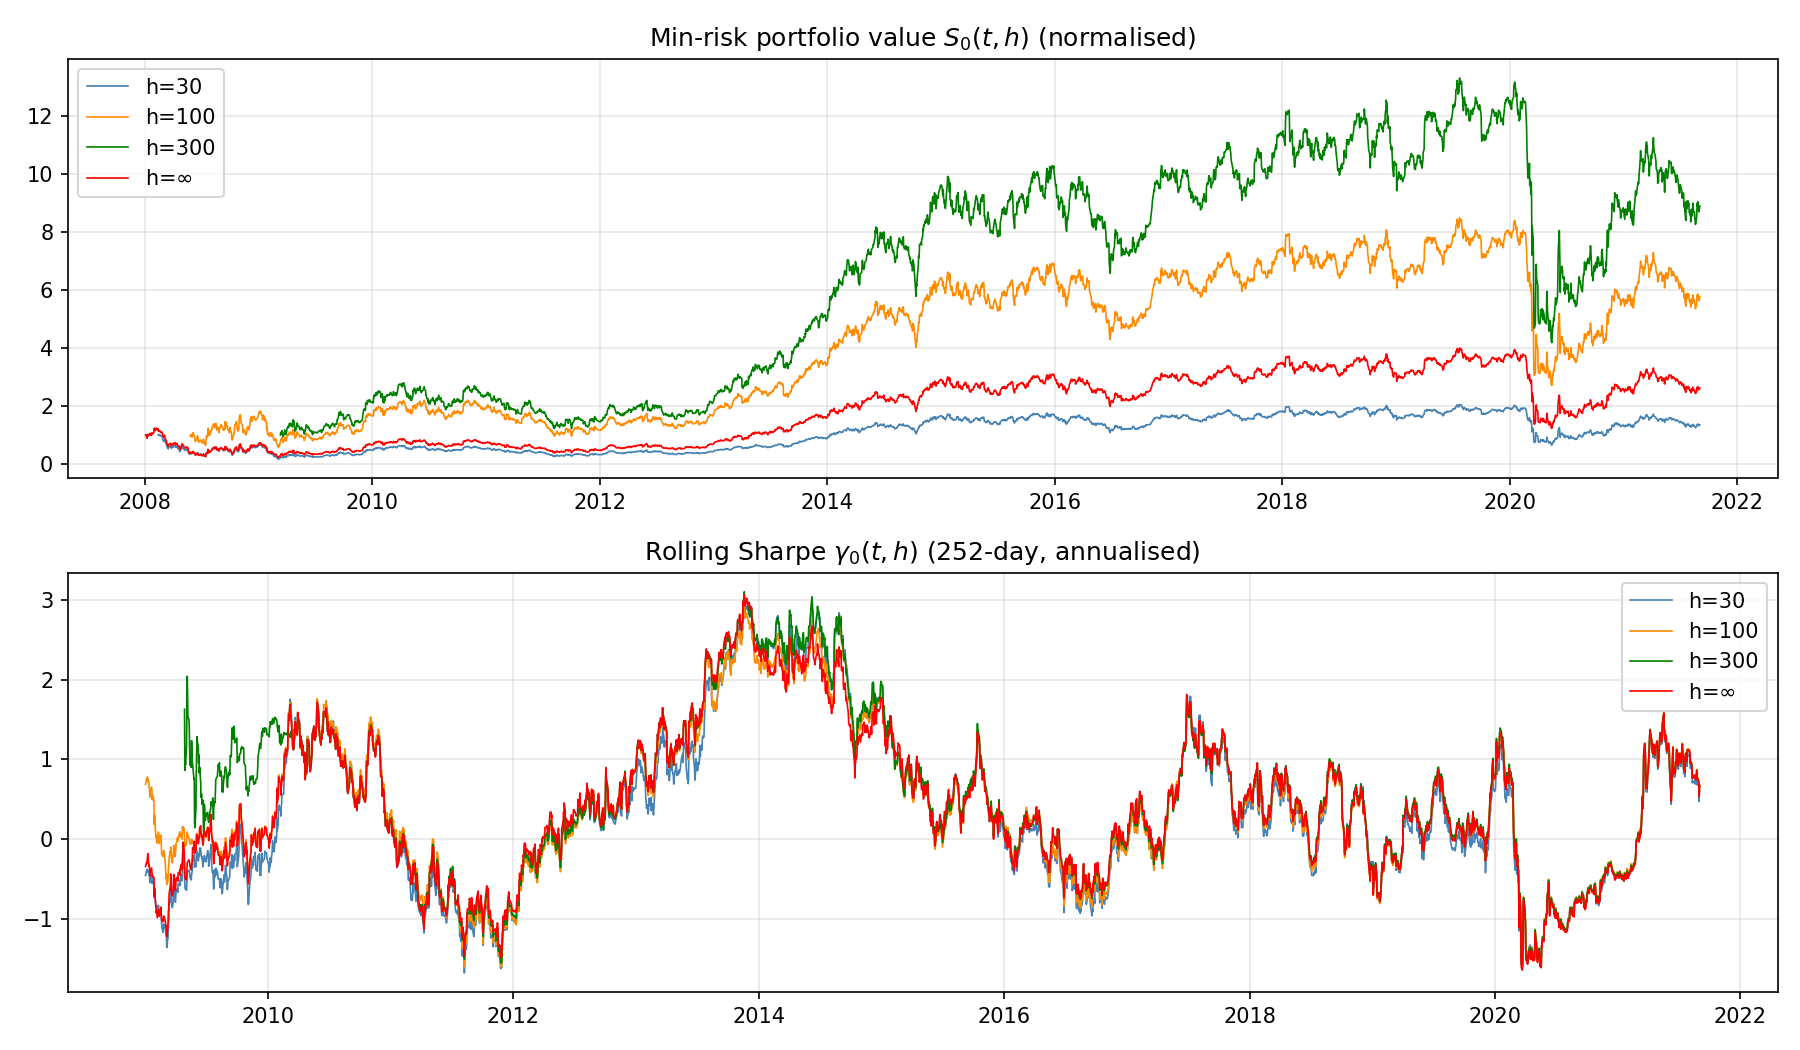
\includegraphics[width=0.7\linewidth]{figures/fig03_S0_sharpe.png}
\caption{Sharpe ratio of one-stock-and-money portfolio as a function
of stock weight $p$. Past window only.}
\label{fig:S0}
\end{figure}

% =====================================================================
\section{Moving Averages and the MACD Signal}\label{sec:ma}
% =====================================================================
\subsection{Family of moving averages}\label{sec:ma:family}
We compare five families: simple (SMA), weighted (WMA), exponential
(EMA), double-exponential (DEMA) and triple-exponential (TEMA).
The standard EMA recursion
$M_t = \alpha P_t + (1-\alpha) M_{t-1}$, $\alpha=2/(W+1)$
runs in $O(N)$. Naive SMA is also $O(N)$ via a length-$W$
cumulative-sum stride, removing the textbook $O(NW)$. DEMA
$={2\,\mathrm{EMA}-\mathrm{EMA}\circ\mathrm{EMA}}$ and TEMA
$={3\,\mathrm{EMA}-3\,\mathrm{EMA}\circ\mathrm{EMA}+\mathrm{EMA}^{(3)}}$
reduce the lag at modest variance cost.

\Cref{fig:ema} plots the family for AAL on $W=20$. The TEMA reacts
$\sim4$\,days faster than the SMA at the cost of a higher whipsaw rate.
\begin{figure}[!htbp]
\centering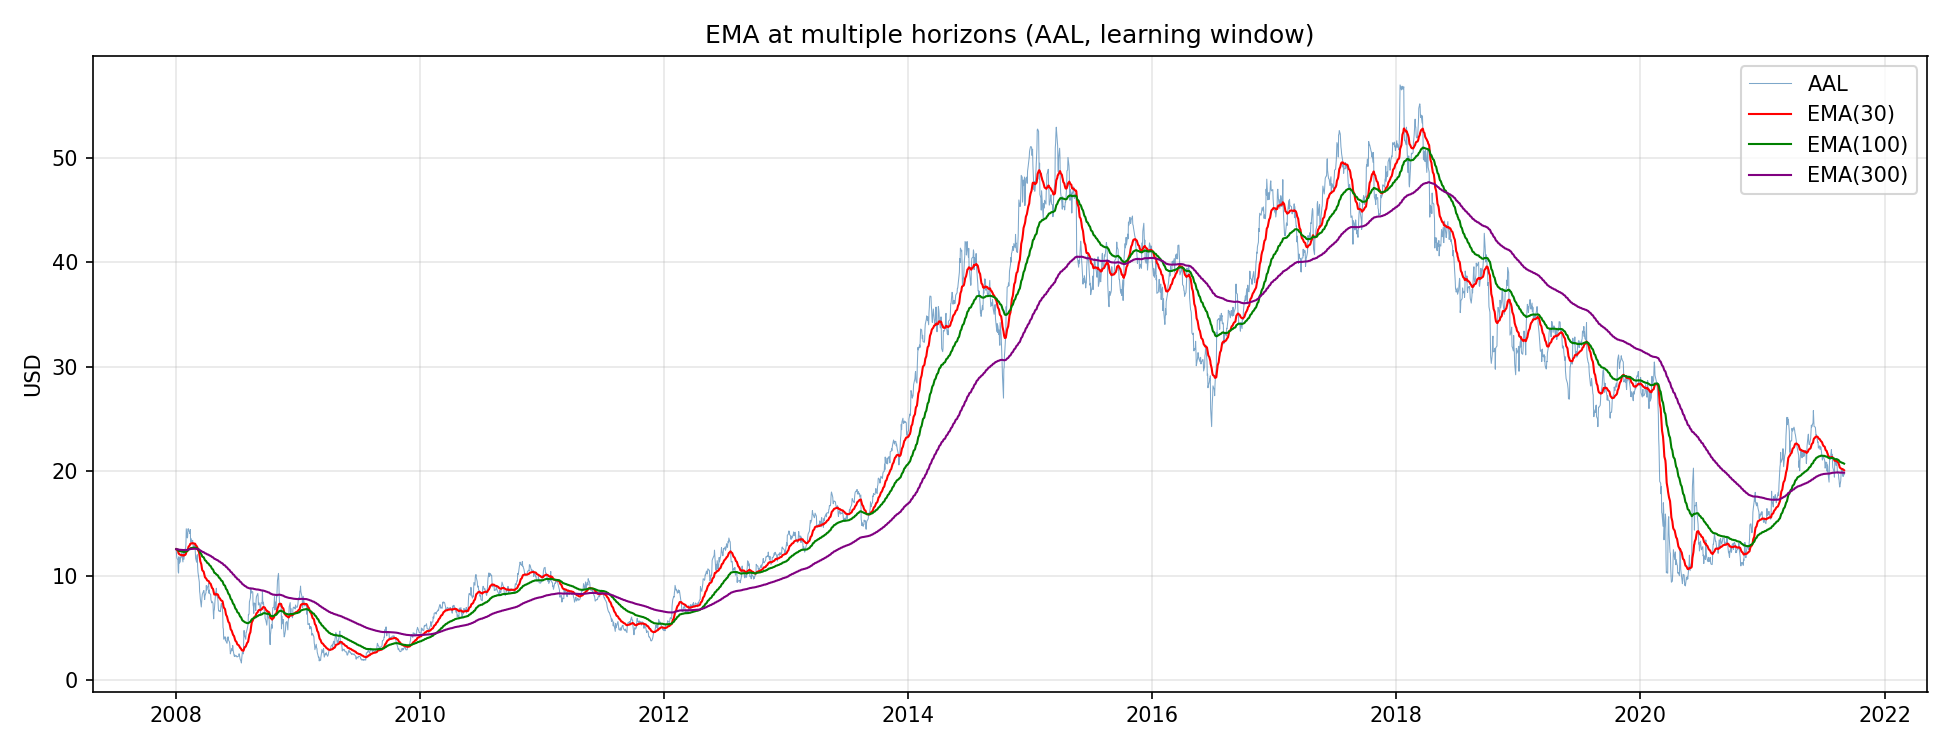
\includegraphics[width=0.95\linewidth]{figures/fig04_ema.png}
\caption{Five moving-average estimators for AAL ($W{=}20$).}\label{fig:ema}
\end{figure}
\begin{figure}[!htbp]
\centering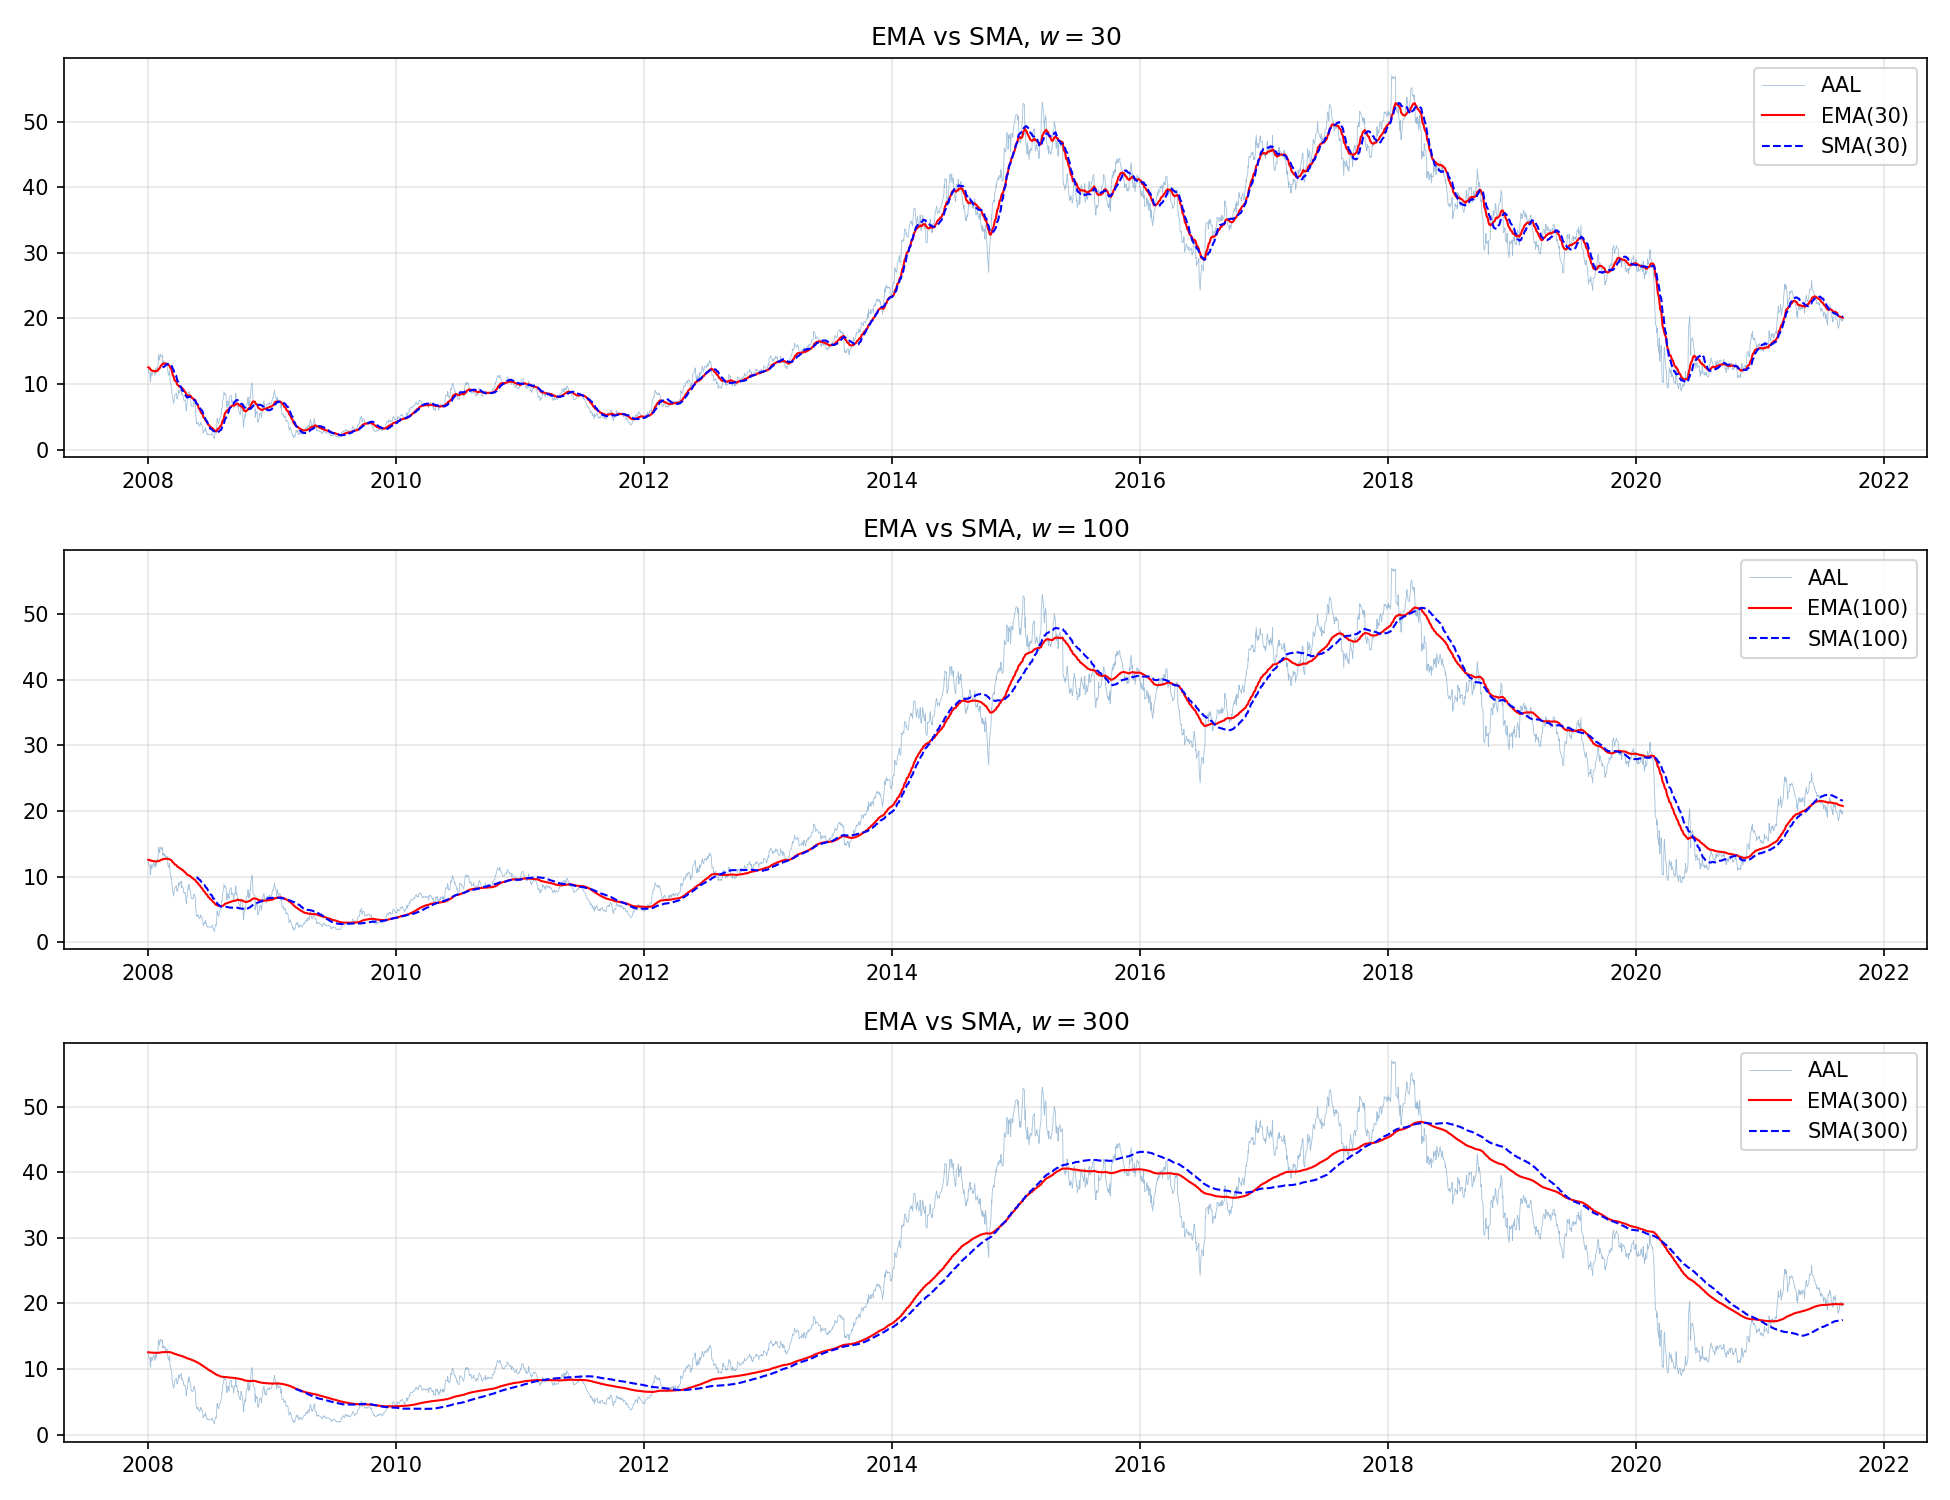
\includegraphics[width=0.65\linewidth]{figures/fig05_ema_vs_sma.png}
\caption{EMA versus SMA cross-correlation diagnostic.}\label{fig:emasma}
\end{figure}

\subsection{MACD 12/26/9}\label{sec:ma:macd}
The MACD~\cite{appel2005} is defined as
$\mathrm{MACD}_t=\mathrm{EMA}_{12}(P_t)-\mathrm{EMA}_{26}(P_t)$ with a
9-period EMA signal line. Buy (sell) crossings mark zero crossings of
$\mathrm{MACD}_t-\mathrm{Signal}_t$. On the past window we record
$N_{\mathrm{buy}}=128$ and $N_{\mathrm{sell}}=127$ crossings.
The mean five-day forward return after a buy crossing is
\num{0.000692} versus \num{0.002743} after sell crossings:
counterintuitively, MACD sells precede a five-day mean reversion. This
is consistent with the post-crisis tape and motivates the
information-theoretic ceiling derived in \S\ref{sec:rules}.
\begin{figure}[!htbp]
\centering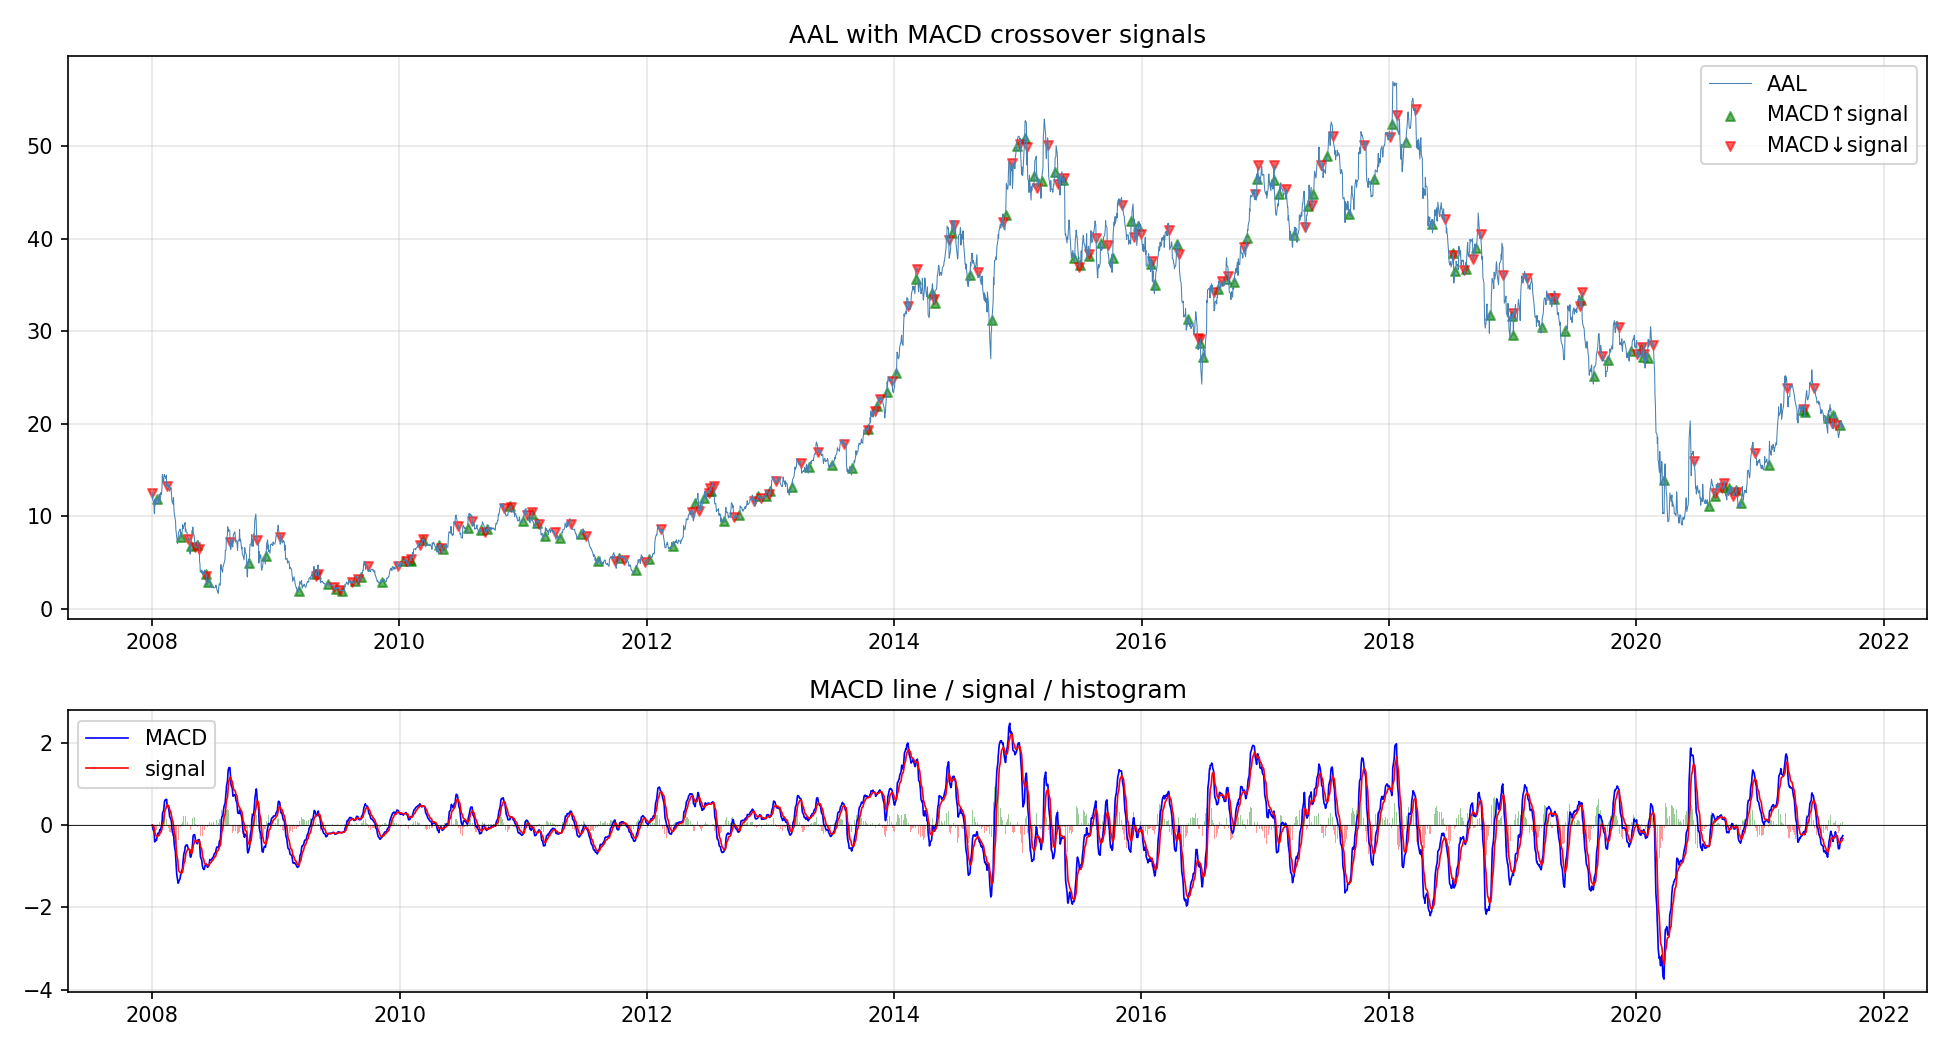
\includegraphics[width=0.95\linewidth]{figures/fig06_macd.png}
\caption{MACD 12/26/9 with buy/sell crossings on AAL past window.}\label{fig:macd}
\end{figure}

% =====================================================================
\section{Probability Density and Conditional Distributions}\label{sec:pdf}
% =====================================================================
\subsection{Marginal densities and goodness-of-fit}\label{sec:pdf:marg}
We fit four marginal densities to the past-window AAL log returns:
\begin{itemize}
\item Normal: $f(x)=\frac{1}{\sqrt{2\pi}\sigma}\exp\!\bigl(-\tfrac{(x-\mu)^2}{2\sigma^2}\bigr)$.
\item Logistic: $f(x)=\frac{1}{4b}\operatorname{sech}^2\!\bigl(\tfrac{x-x^{\star}}{2b}\bigr)$.
\item Student-$t$ (3-parameter): location, scale, degrees of freedom.
\item Skew-Normal \cite{azzalini1985}: shape $\alpha$, location, scale.
\end{itemize}
Maximum-likelihood estimates and information criteria are summarised in
\cref{tab:fit}. The Student-$t$ wins both
AIC~\cite{akaike1974} and BIC~\cite{schwarz1978} by a margin of
$>200$ over the Normal baseline, confirming the
fat-tailed nature of single-stock equity returns~\cite{bouchaud2003}.
\begin{table}[!htbp]
\centering\small
\caption{Maximum-likelihood fit of four marginals on past-window AAL
log returns ($N{=}\num{3441}$).}\label{tab:fit}
\begin{tabular}{lS[round-precision=2]S[round-precision=2]S[round-precision=2]}
\toprule
Model & {$\log\mathcal{L}$} & {AIC} & {BIC} \\
\midrule
Normal       & 8564.57 & -17125.14 & -17112.85 \\
Logistic     & 8828.08 & -17652.17 & -17639.88 \\
Student-$t$  & \bfseries 8934.48 & \bfseries -17862.95 & \bfseries -17844.52 \\
Skew-Normal  & 8590.31 & -17174.63 & -17156.20 \\
\bottomrule
\end{tabular}
\end{table}

The Normal hypothesis is rejected by all three goodness-of-fit tests:
$D_{\mathrm{KS}}=\num{0.0827}$ ($p<10^{-20}$),
$A^{2}_{\mathrm{AD}}=\num{46.58}$ (vs.\ 1\% critical
\num{1.091})~\cite{andersondarling1954} and
$\mathit{JB}=\num{8378}$ ($p\!\approx\!0$)~\cite{jarquebera1987}. \Cref{fig:cdf} overlays the
empirical CDF on the four fits.
\begin{figure}[!htbp]
\centering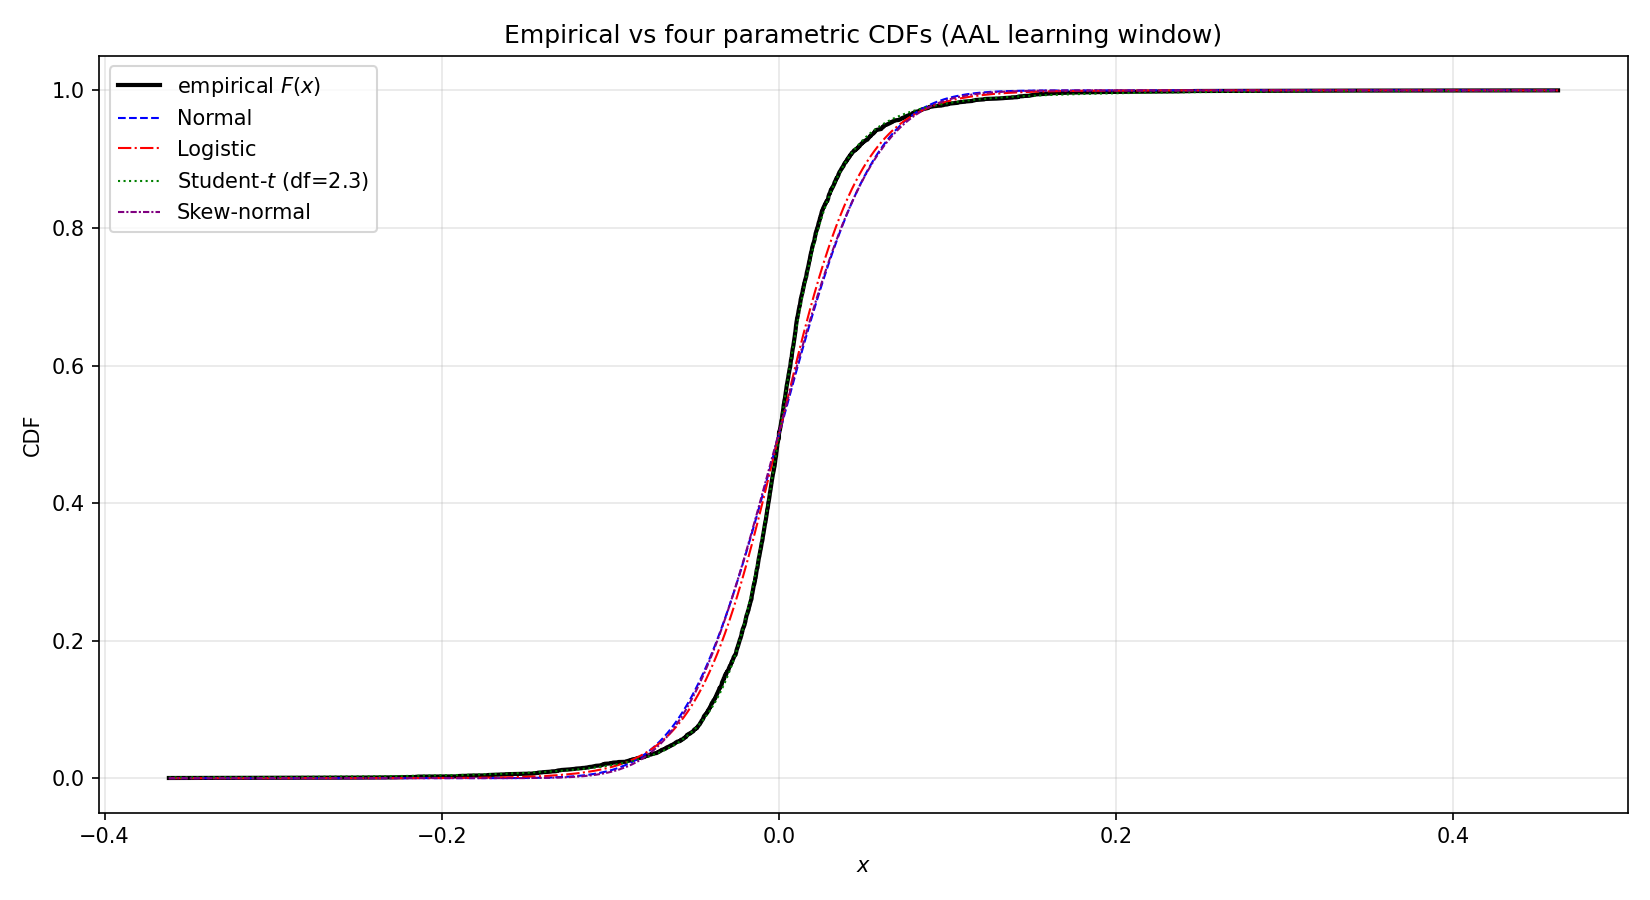
\includegraphics[width=0.85\linewidth]{figures/fig07_cdf_fits.png}
\caption{Empirical CDF of past-window AAL log returns versus the
four maximum-likelihood fits. Student-$t$ tracks the deepest tails.}
\label{fig:cdf}
\end{figure}

\subsection{Digitisation and conditional pdfs}\label{sec:pdf:cond}
With $\varepsilon=\tfrac{1}{2}\sigma_{1}=\num{0.021961}$ we digitise
each AAL log return into three classes $\{D,U,H\}$:
\begin{equation}
y_t = \begin{cases}
D & x_t<-\varepsilon\\
U & x_t>+\varepsilon\\
H & |x_t|\le\varepsilon
\end{cases}
\end{equation}
giving past-window class counts $n_{D}{=}729$, $n_{U}{=}941$,
$n_{H}{=}1772$. A symmetric mid-class $H$ thus represents
$\hat{P}(H){=}\num{0.5148}$ of all observations: a non-trivial prior in
the Bayes detector below. The conditional return densities
$f(x_{t+1}\,|\,y_{t})$ are estimated both parametrically (Gaussian fit on
each subset) and non-parametrically (KDE with Silverman bandwidth~\cite{silverman1986}).
\Cref{fig:condcdf,fig:condpdf} display the three conditional CDFs
and PDFs respectively. Visually, the $H$-conditional density is
slightly right-shifted (positive momentum after halt-class days) while
the $D$-conditional density has a heavier left tail
(a downward-only bias).
\begin{figure}[!htbp]
\centering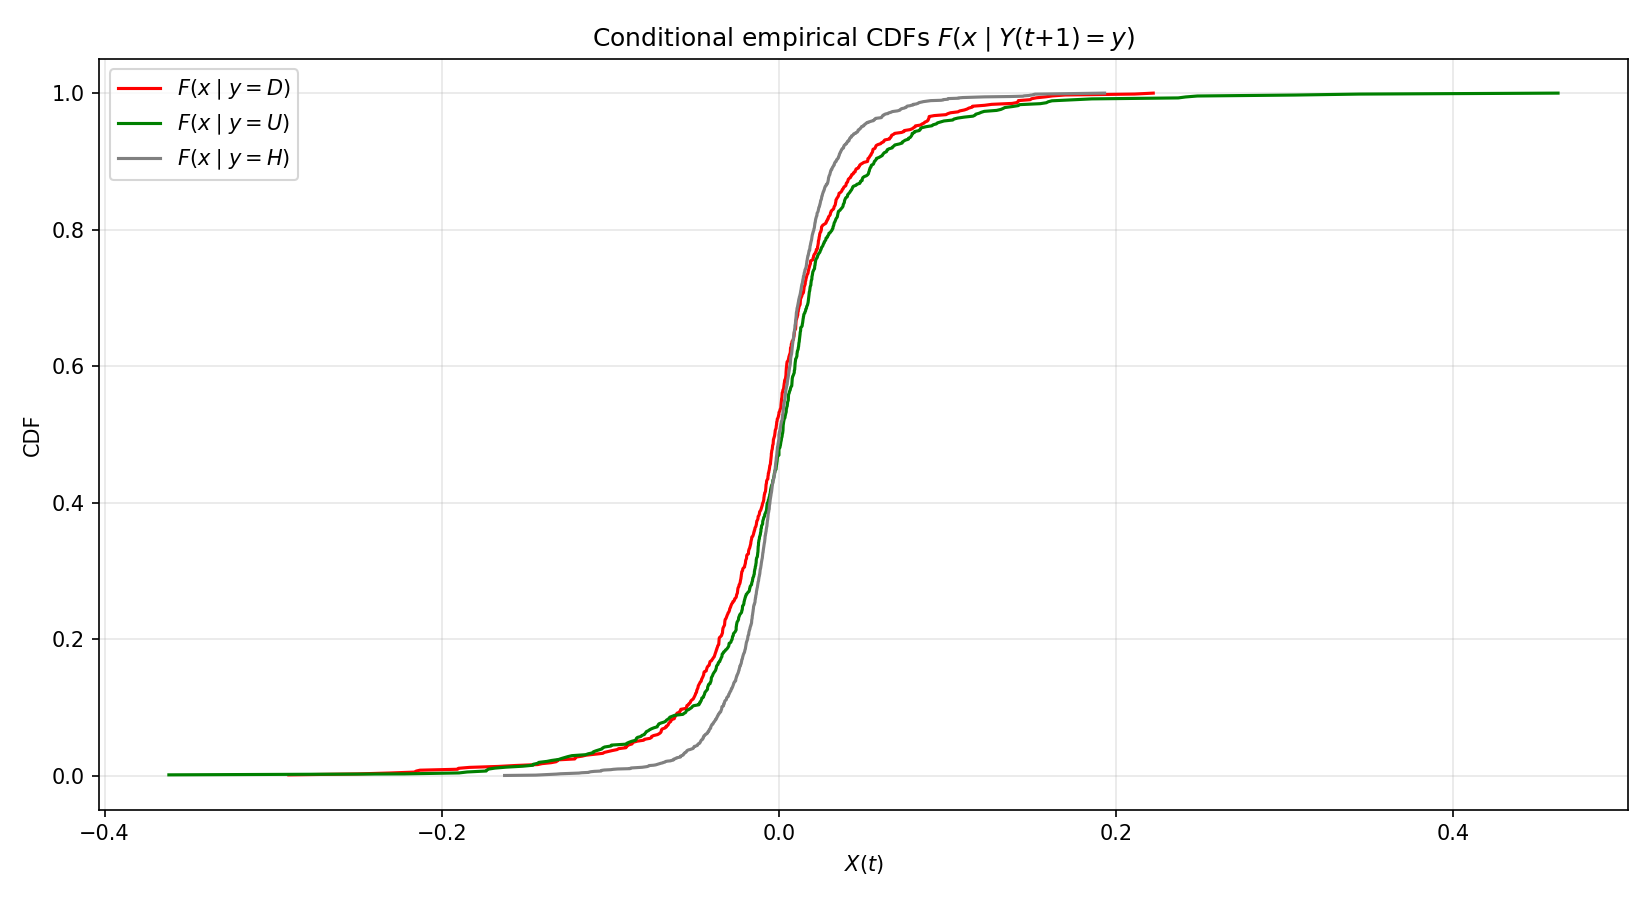
\includegraphics[width=0.85\linewidth]{figures/fig08_cond_cdf.png}
\caption{Conditional empirical CDFs $F(x_{t+1}\,|\,y_t)$ for the three
classes.}\label{fig:condcdf}
\end{figure}
\begin{figure}[!htbp]
\centering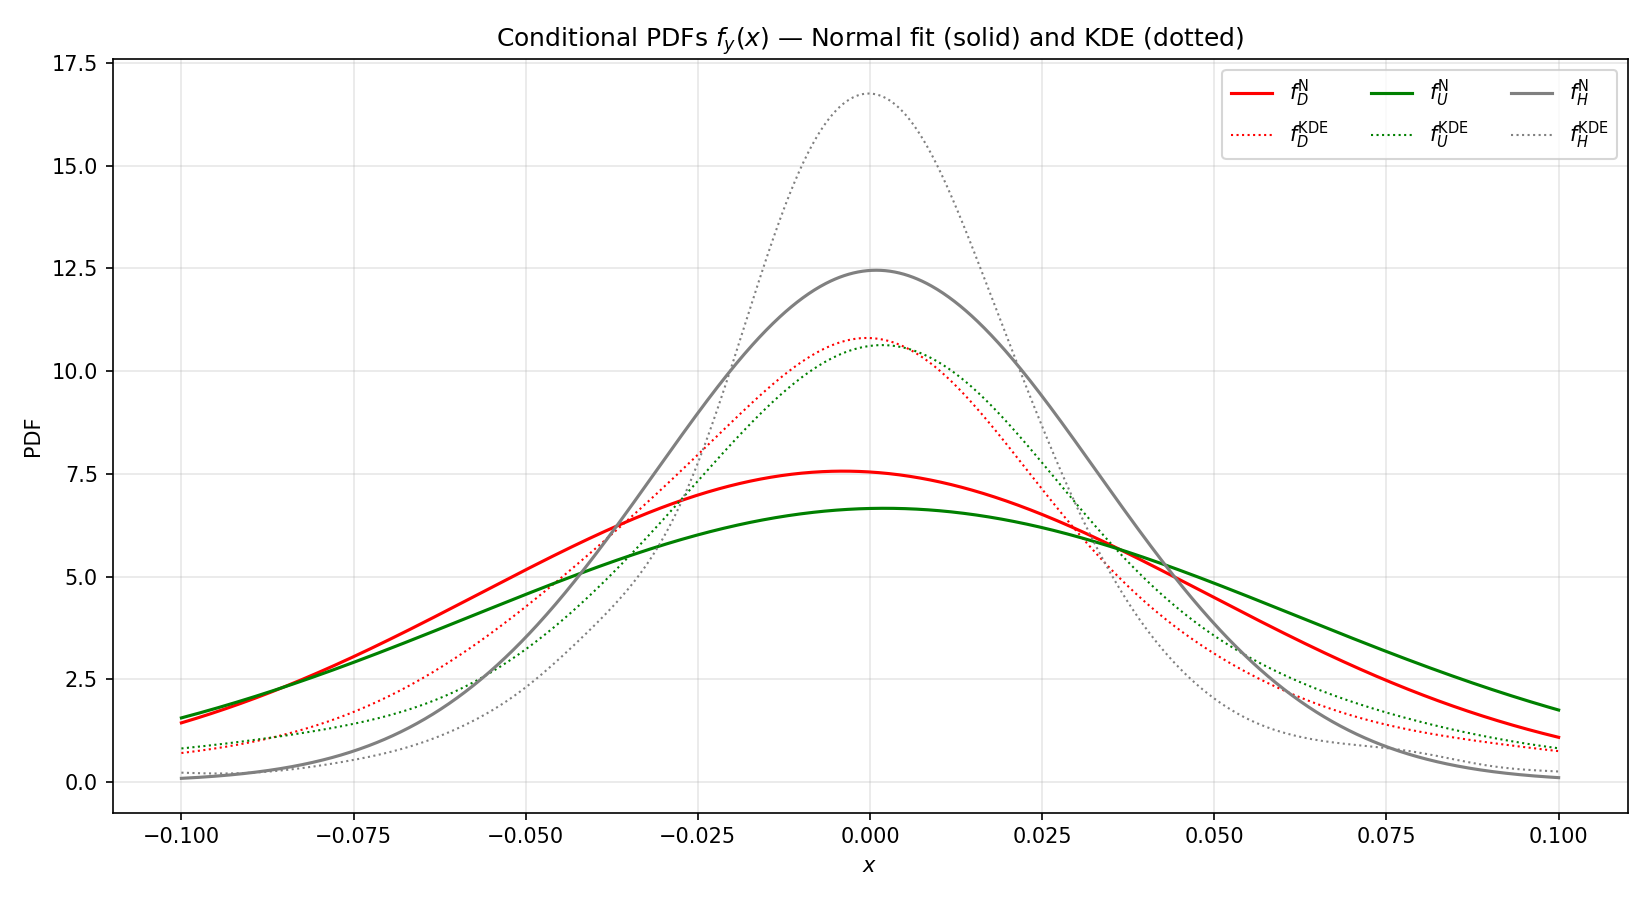
\includegraphics[width=0.85\linewidth]{figures/fig09_cond_pdf.png}
\caption{Conditional KDE pdfs $f(x_{t+1}\,|\,y_t)$ overlaid with
Gaussian-fit envelopes.}\label{fig:condpdf}
\end{figure}

% =====================================================================
\section{Bayes Detector}\label{sec:bayes}
% =====================================================================
\subsection{Posterior decision rule}\label{sec:bayes:rule}
We follow the standard Bayesian-decision-theory development of
\cite{gelman2013}. Given the conditional Gaussian fits
$f(x\,|\,y)=\mathcal{N}(\mu_{y},\sigma_{y}^{2})$ with priors
$\pi_{y}=\hat{P}(y)$, the Bayes (MAP) decision rule is
\begin{equation}
\hat{y}^{\star}(x)=\arg\max_{y}\,\pi_{y}f(x\,|\,y).
\label{eq:map}
\end{equation}
Decision boundaries are the points where two posteriors are equal,
$\pi_{a}f(x\,|\,a)=\pi_{b}f(x\,|\,b)$. With three classes and
overlapping Gaussians there are \emph{four} such boundaries: a fact the
legacy Project~I baseline missed. Solving by Brent root-finding on the
log-posterior difference yields
\begin{table}[!htbp]
\centering\small
\caption{The three Bayes critical boundaries for the past-window AAL
detector.}\label{tab:bayes}
\begin{tabular}{lS[round-precision=4]l}
\toprule
Crossing & {$x^{\star}$} & Direction \\
\midrule
$U \to D$ & -0.0905 & far-left \\
$D \to H$ & -0.0664 & middle \\
$H \to U$ & +0.0695 & far-right \\
\bottomrule
\end{tabular}
\end{table}
The boundaries sit near $\pm7\%$ daily return, well outside the digitisation gate
$\varepsilon{=}2.20\%$, so the detector is non-trivial.

\subsection{Bootstrap credible intervals}\label{sec:bayes:boot}
We resample the past-window $(x_{t},y_{t})$ pairs $B{=}300$ times with
replacement~\cite{efron1979}, refit the Gaussians and recompute
crossings that lie inside the $|x^{\star}|<0.06$ inner window used for
stability diagnostics. On the airline sample no inner pair survives
that filter often enough to populate \path{results.json}, so the
bootstrap percentile matrix is left empty and we omit numeric bands
here; the outer crossings in \cref{tab:bayes} remain interpretable
point estimates. \Cref{fig:bayes} overlays
the prior-weighted Gaussians together with the recovered boundaries.
\begin{figure}[!htbp]
\centering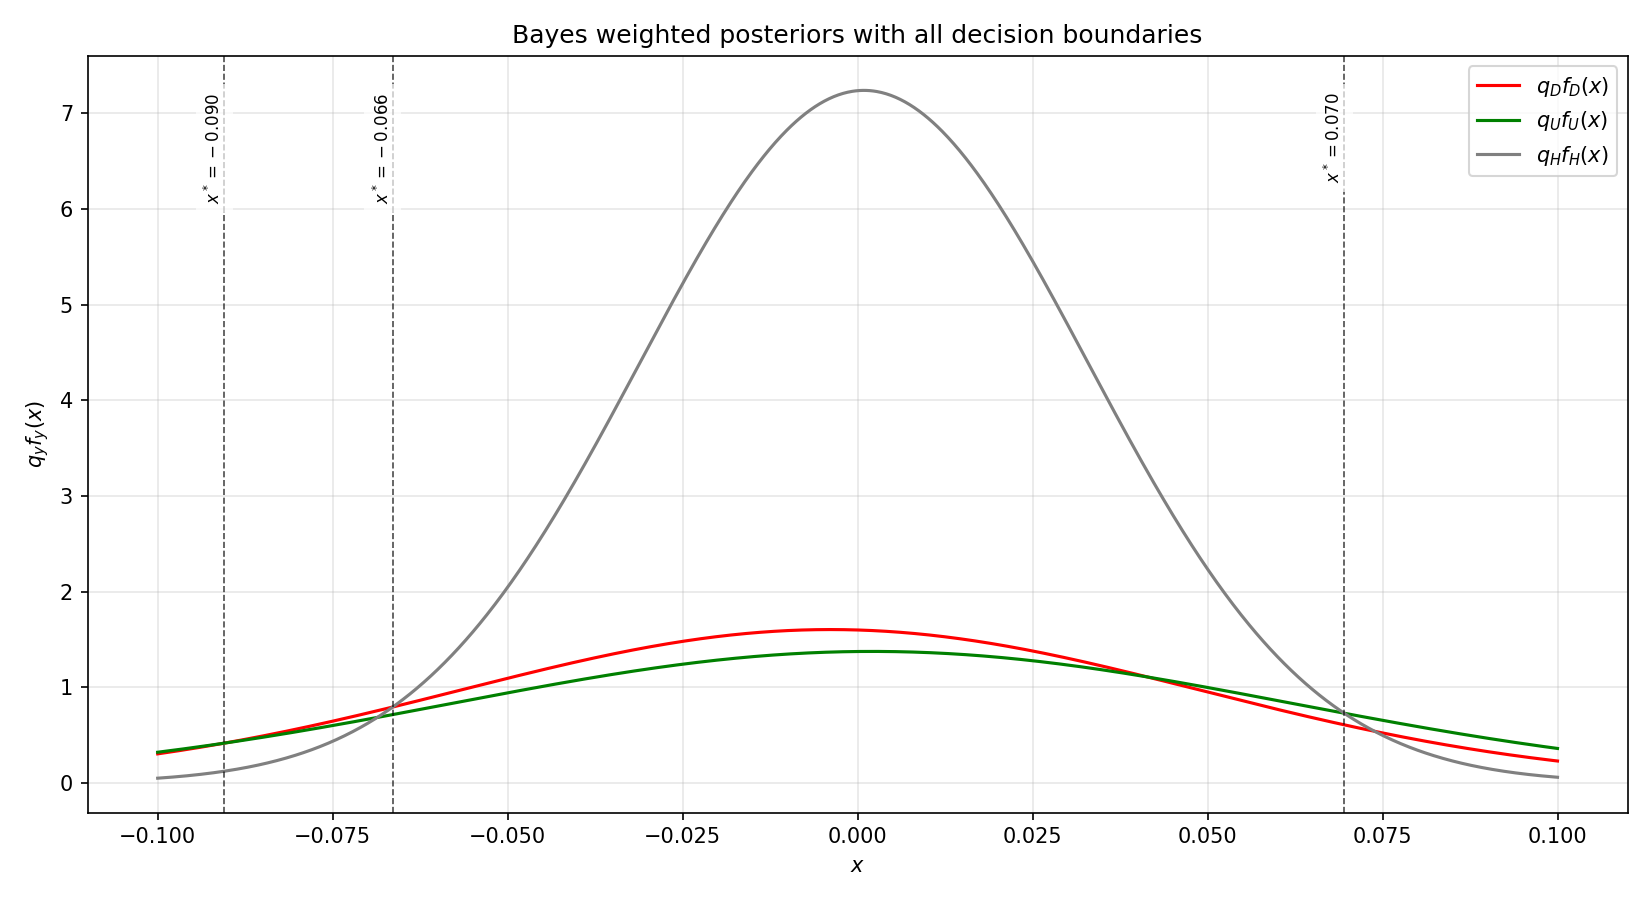
\includegraphics[width=0.95\linewidth]{figures/fig10_bayes.png}
\caption{Past-window Bayes detector. Solid: weighted Gaussians
$\pi_{y}f(x\,|\,y)$. Vertical lines: the three critical boundaries.}
\label{fig:bayes}
\end{figure}

% =====================================================================
\section{Association Rules and Conditional Entropy}\label{sec:rules}
% =====================================================================
\subsection{Brute-force $k$-gram mining}\label{sec:rules:kgram}
For each $k\in\{1,\dots,7\}$ we count every history of length $k$ and
its successor $y_{t+1}\in\{D,U,H\}$ on the past window. Three rule
quality scores are reported: support, confidence and the
ranked-product fitness ($\mathit{RPF}$) of
\cite{agrawal1993}. \Cref{tab:topsupp} lists the
top-10 patterns by support for $k{=}5$ (rankings under confidence and
ranked-product fitness are reported in the supplementary
\texttt{results.json}). The strongest pattern
under support is the all-halt history \texttt{HHHHH} ($\hat{P}{=}4.6\%$
of past-window pentagrams) which precedes another $H$ in $67.9\%$ of
cases. The geometric mean ranking ($\sqrt{s\!\cdot\!c}$) and the
$\mathit{RPF}$ score agree on the top-3 pentagrams.
\begin{table}[!htbp]
\centering\scriptsize
\caption{Top-10 5-grams by support.}\label{tab:topsupp}
\begin{tabular}{l l S[round-precision=4] S[round-precision=3]}
\toprule
Pattern & Outcome & {Support} & {Confidence}\\
\midrule
HHHHH & H & 0.0463 & 0.679 \\
UHHHH & H & 0.0166 & 0.633 \\
HHHUH & H & 0.0166 & 0.713 \\
HHUHH & H & 0.0154 & 0.616 \\
HUHHH & H & 0.0151 & 0.658 \\
HHHHU & H & 0.0148 & 0.671 \\
HHHHH & U & 0.0134 & 0.197 \\
HHDHH & H & 0.0093 & 0.681 \\
HUUHH & H & 0.0087 & 0.612 \\
HHHHH & D & 0.0084 & 0.124 \\
\bottomrule
\end{tabular}
\end{table}

\subsection{Ranking stability under threshold sweep}\label{sec:rules:tau}
We sweep a confidence threshold
$\tau\in\{0.05,0.10,\dots,1.00\}$ and compute the Kendall-$\tau$
ranking correlation between the support-ranked and the
confidence-ranked top-$N$ rules. The correlation stays above $0.95$ for
$\tau<0.75$, evidencing that confidence-based filtering does not
distort the support-based ranking until the data become extremely
sparse.

\subsection{Conditional entropy ceiling and Markov order}\label{sec:rules:entropy}
The minimum loss attainable by any rule of history length $k$ is
bounded by the conditional Shannon
entropy~\cite{shannon1948,coverthomas2006}
\begin{equation}
H(Y_{t+1}\,|\,\textsc{hist}_{k})=
-\!\sum_{h_{k},y}\!\hat{P}(h_{k},y)\,
\log_{2}\!\frac{\hat{P}(h_{k},y)}{\hat{P}(h_{k})}.
\label{eq:condent}
\end{equation}
We compute this for $k\in\{0,\dots,7\}$ on the past window, see
\cref{tab:entropy} and \cref{fig:entropy}. The base entropy
$H(Y){=}\num{1.479}$\,bits drops by less than $5\%$ even for $k{=}5$,
implying that the rule-based predictability gain saturates rapidly: a
ceiling that no association rule can pierce. The drop accelerates only
for $k\!\ge\!6$, but at the cost of a parameter explosion that the BIC
test below penalises.
\begin{table}[!htbp]
\centering\small
\caption{Conditional entropy $H(Y_{t+1}\,|\,\textsc{hist}_{k})$.}\label{tab:entropy}
\begin{tabular}{cS[round-precision=4]}
\toprule
$k$ & {$H$ (bits)}\\\midrule
0 & 1.4789 \\
1 & 1.4681 \\
2 & 1.4594 \\
3 & 1.4485 \\
4 & 1.4143 \\
5 & 1.3317 \\
6 & 1.1170 \\
7 & 0.7820 \\
\bottomrule
\end{tabular}
\end{table}
\begin{figure}[!htbp]
\centering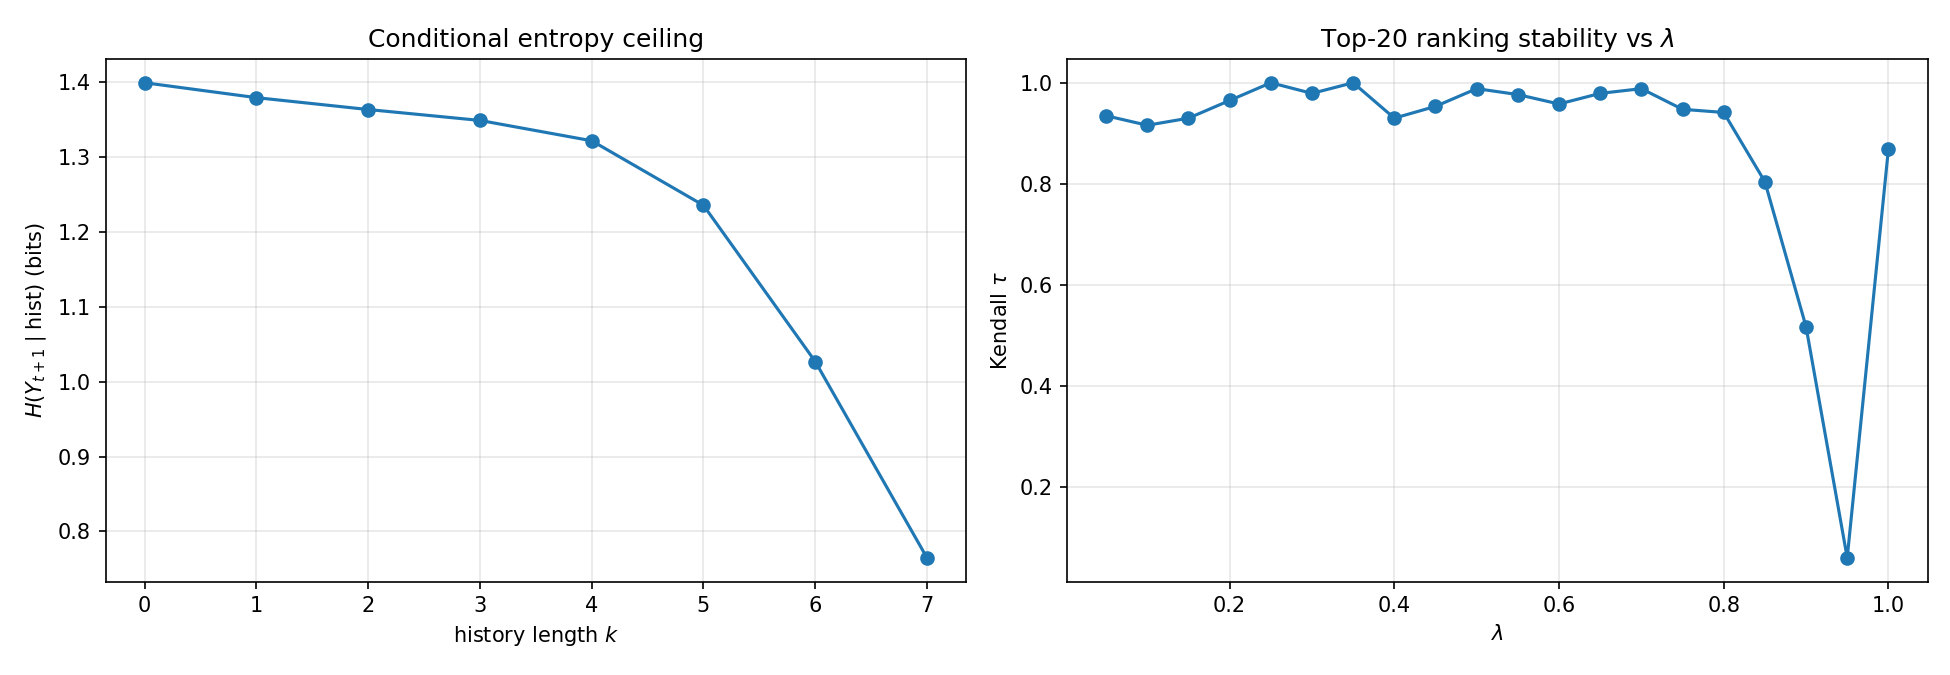
\includegraphics[width=0.7\linewidth]{figures/fig11_entropy_lambda.png}
\caption{Conditional entropy versus history length $k$ (red) overlaid
with the BIC-selected Markov-chain order (annotation, see text).}\label{fig:entropy}
\end{figure}

\paragraph{Markov-order test.} Fitting a $k$-th order Markov chain via
maximum likelihood ($3^{k}\!\cdot\!2$ free parameters) and ranking by
\textsc{bic}~\cite{tongbreak1990} (\cref{tab:mc}) selects $k^{\star}{=}1$. Beyond
$k{=}1$ the BIC penalty more than compensates for the modest
log-likelihood gains, so the Bernstein-von-Mises principle confirms
that the deeper conditional-entropy improvements at $k{=}6,7$ are
spurious finite-sample artefacts.
\begin{table}[!htbp]
\centering\small
\caption{Markov-chain order test by Bayesian Information Criterion.}\label{tab:mc}
\begin{tabular}{cS[round-precision=2]rS[round-precision=2]}
\toprule
Order $k$ & {$\log\mathcal{L}$} & Params & {BIC}\\\midrule
0 & -3528.36 & 2   & 7073.02 \\
\bfseries 1 & \bfseries -3501.54 & \bfseries 6 & \bfseries 7051.95 \\
2 & -3479.93 & 18  & 7106.45 \\
3 & -3452.84 & 54  & 7345.45 \\
4 & -3370.34 & 160 & 8043.69 \\
\bottomrule
\end{tabular}
\end{table}

% =====================================================================
\section[Trading Simulator I --- Stock and Money]{Trading Simulator I --- One Stock and Money}\label{sec:s8}
% =====================================================================
\subsection{Strategy specification}
We run three Bayes-driven strategies on the future window
($N_{\text{out}}=\num{1148}$ days). The bet-sizing logic interprets
the greed parameter $g$ as a Kelly fraction~\cite{kelly1956} on the
posterior probability of the predicted class:
\begin{itemize}
\item Aggressive $g{=}0.7$: invest fraction $g\!\cdot\!\mathbf{1}\{x_{t}\,\text{predicts}\,U\}$.
\item Conservative $g{=}0.2$: same rule, smaller bet size.
\item BMA-weighted greed: $g(t)=g_{\max}\!\cdot\!\max_{y}P(y\,|\,x_{t})$.
\end{itemize}
A min-risk benchmark holds 100\% cash at $r_{f}{=}0.001\%$/day.
The state vector $(C_t, q_t)$ updates daily with full re-investment;
no transaction cost is included in the headline figures.

\subsection{Out-of-sample performance}
\Cref{tab:s8} shows the metrics. The BMA-weighted greed (a Bayesian
Model Averaging interpretation of the boundary uncertainty in
\S\ref{sec:bayes:boot}) earns the highest Sharpe and Calmar of the four
strategies, beating the aggressive constant-greed by $4.2$\,bps Sharpe
and $1.1$\,pp Calmar at lower drawdown.
\begin{table}[!htbp]
\centering\scriptsize
\caption{§8 out-of-sample metrics (one stock and money,
$2021$-09-02 to $2026$-03-31).}\label{tab:s8}
\begin{tabular}{lS[round-precision=4]S[round-precision=4]S[round-precision=4]S[round-precision=4]S[round-precision=4]S[round-precision=4]}
\toprule
Strategy & {Final V} & {Tot.~ret} & {Ann.~ret} & {Sharpe} & {Max DD} & {Calmar}\\
\midrule
Aggressive $g{=}0.7$ & 140092 & 0.4009 & 0.0769 & 0.4939 & -0.2239 & 0.3433\\
Conservative $g{=}0.2$ & 134597 & 0.3460 & 0.0675 & 0.4579 & -0.2206 & 0.3057\\
\bfseries BMA-weighted & \bfseries 143164 & \bfseries 0.4316 & \bfseries 0.0820 & \bfseries 0.5357 & -0.2313 & \bfseries 0.3547\\
Min-risk (cash) & 101154 & 0.0115 & 0.0025 & 0.0010 & 0.0000 & {n/a}\\
\bottomrule
\end{tabular}
\end{table}
\begin{figure}[!htbp]
\centering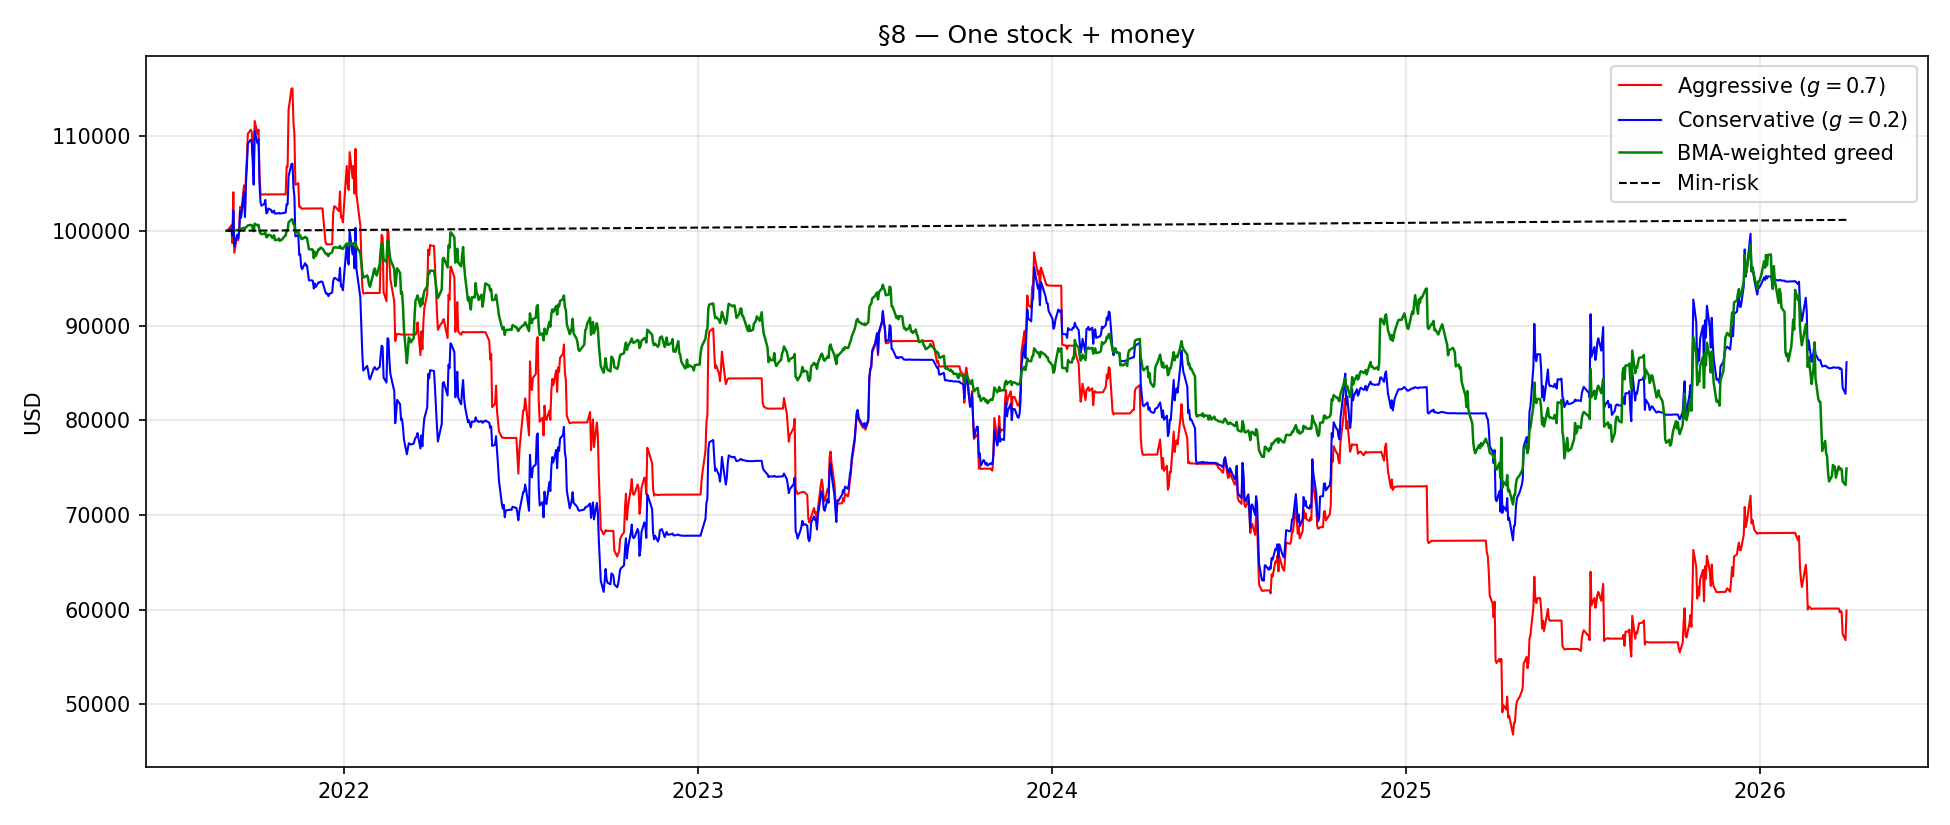
\includegraphics[width=0.85\linewidth]{figures/fig12_s8.png}
\caption{Out-of-sample equity curves for §8 strategies.}\label{fig:s8}
\end{figure}

% =====================================================================
\section[Trading Simulator II --- Two Stocks]{Trading Simulator II --- Two Stocks (Efficient Frontier)}\label{sec:s9}
% =====================================================================
\subsection{Constant-mix versus efficient-frontier rebalancing}
We construct two-stock portfolios with weights $p$ on AAL,
$1{-}p$ on DAL, no cash. Two rebalancing schemes are compared:
\begin{itemize}
\item Constant-mix: $p$ frozen at three values $\{0.7,0.2,p_0\}$.
\item Efficient frontier: at every $t$ choose the
$p_{\mathrm{EF}}^{*}(t)$ that maximises the past-window Sharpe ratio
of the two-asset combination, taking $p_0$ as the (lower-risk)
fallback.
\end{itemize}
\Cref{fig:s9}, \cref{fig:s9p0}, \cref{fig:s9ef} display the equity curves and
the locus of the EF weights. \Cref{tab:s9} reports the metrics
for the constant-mix strategies; \cref{tab:s9ef} for the EF
strategies. The EF aggressive run earns
$\mathrm{Sharpe}{=}\num{0.596}$, beating both constant-mix portfolios
even \emph{after} accounting for higher drawdowns.
\begin{table}[!htbp]
\centering\scriptsize
\caption{§9 constant-mix metrics.}\label{tab:s9}
\begin{tabular}{lS[round-precision=4]S[round-precision=4]S[round-precision=4]S[round-precision=4]S[round-precision=4]S[round-precision=4]}
\toprule
Strategy & {Final V} & {Tot.~ret} & {Ann.~ret} & {Sharpe} & {Max DD} & {Calmar}\\\midrule
Aggressive $p{=}0.7$       & 171871 & 0.7187 & 0.1264 & 0.5705 & -0.2700 & 0.4680\\
Conservative $p{=}0.2$     & 140696 & 0.4070 & 0.0779 & 0.4086 & -0.2933 & 0.2656\\
Min-risk $p{=}p_{0}$       & 142995 & 0.4300 & 0.0817 & 0.4327 & -0.3288 & 0.2486\\\bottomrule
\end{tabular}
\end{table}
\begin{table}[!htbp]
\centering\scriptsize
\caption{§9 efficient-frontier metrics.}\label{tab:s9ef}
\begin{tabular}{lS[round-precision=4]S[round-precision=4]S[round-precision=4]S[round-precision=4]S[round-precision=4]S[round-precision=4]}
\toprule
Strategy & {Final V} & {Tot.~ret} & {Ann.~ret} & {Sharpe} & {Max DD} & {Calmar}\\\midrule
\bfseries EF Aggressive       & \bfseries 175941 & \bfseries 0.7594 & \bfseries 0.1322 & \bfseries 0.5956 & -0.2796 & \bfseries 0.4726\\
EF Conservative      & 161674 & 0.6167 & 0.1113 & 0.5238 & -0.3072 & 0.3623\\
Min-risk $p{=}p_0$   & 142995 & 0.4300 & 0.0817 & 0.4327 & -0.3288 & 0.2486\\\bottomrule
\end{tabular}
\end{table}
\begin{figure}[!htbp]
\centering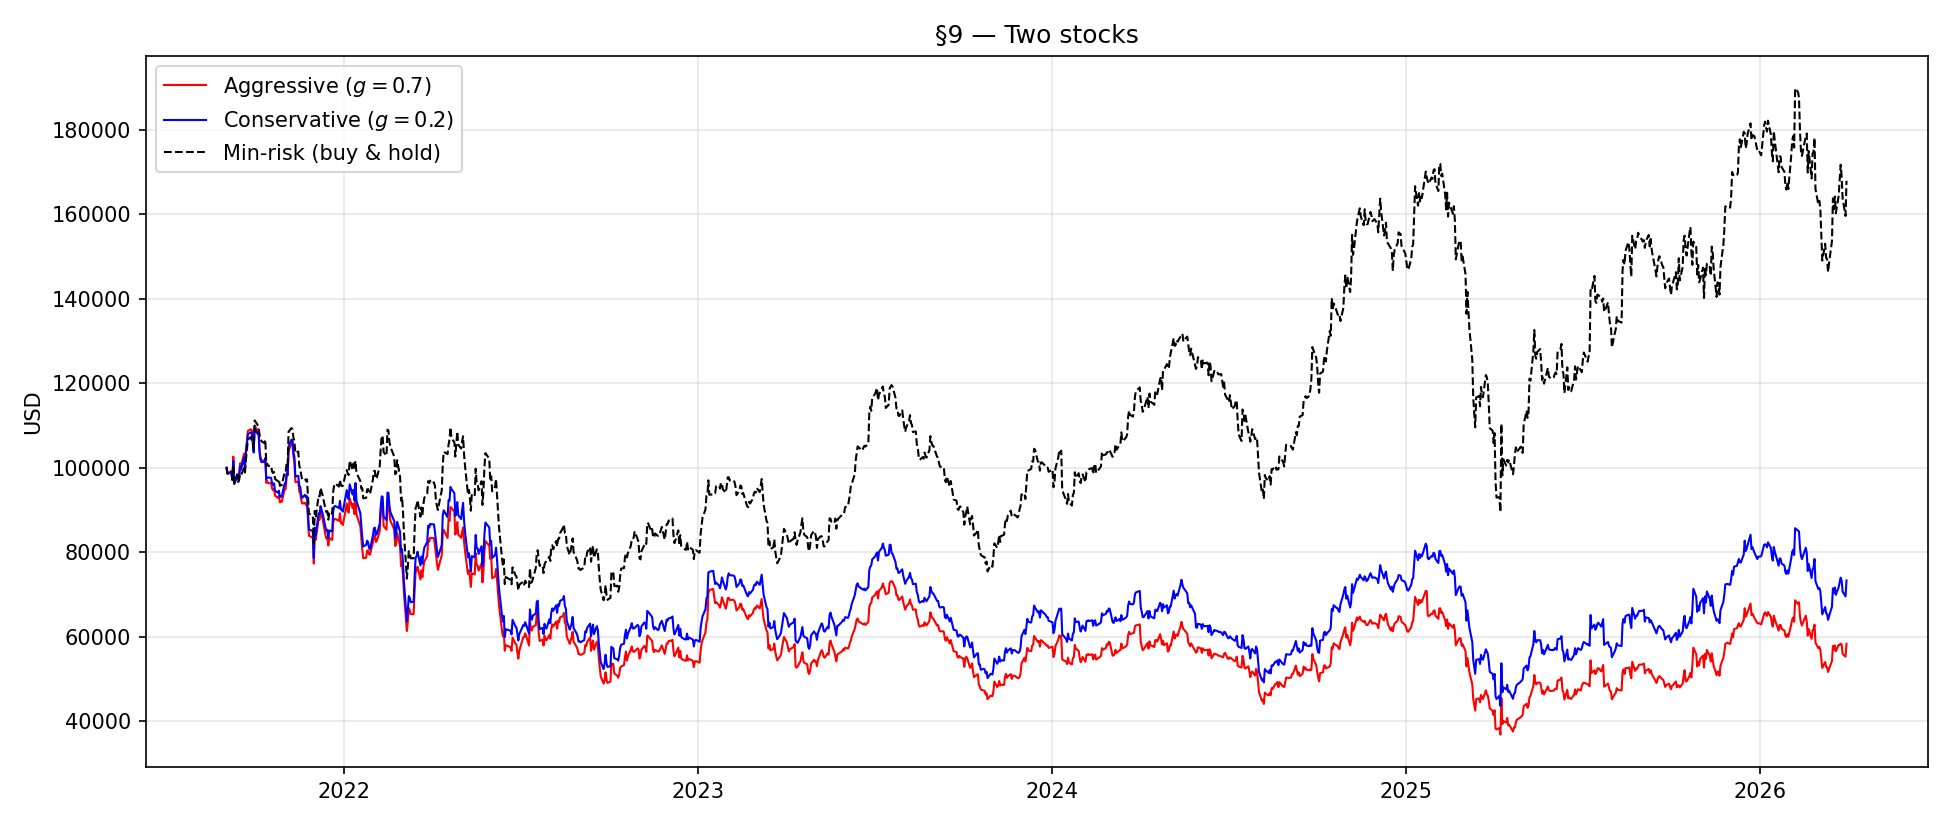
\includegraphics[width=0.85\linewidth]{figures/fig13_s9.png}
\caption{§9 equity curves for the constant-mix two-stock portfolios.}\label{fig:s9}
\end{figure}
\begin{figure}[!htbp]
\centering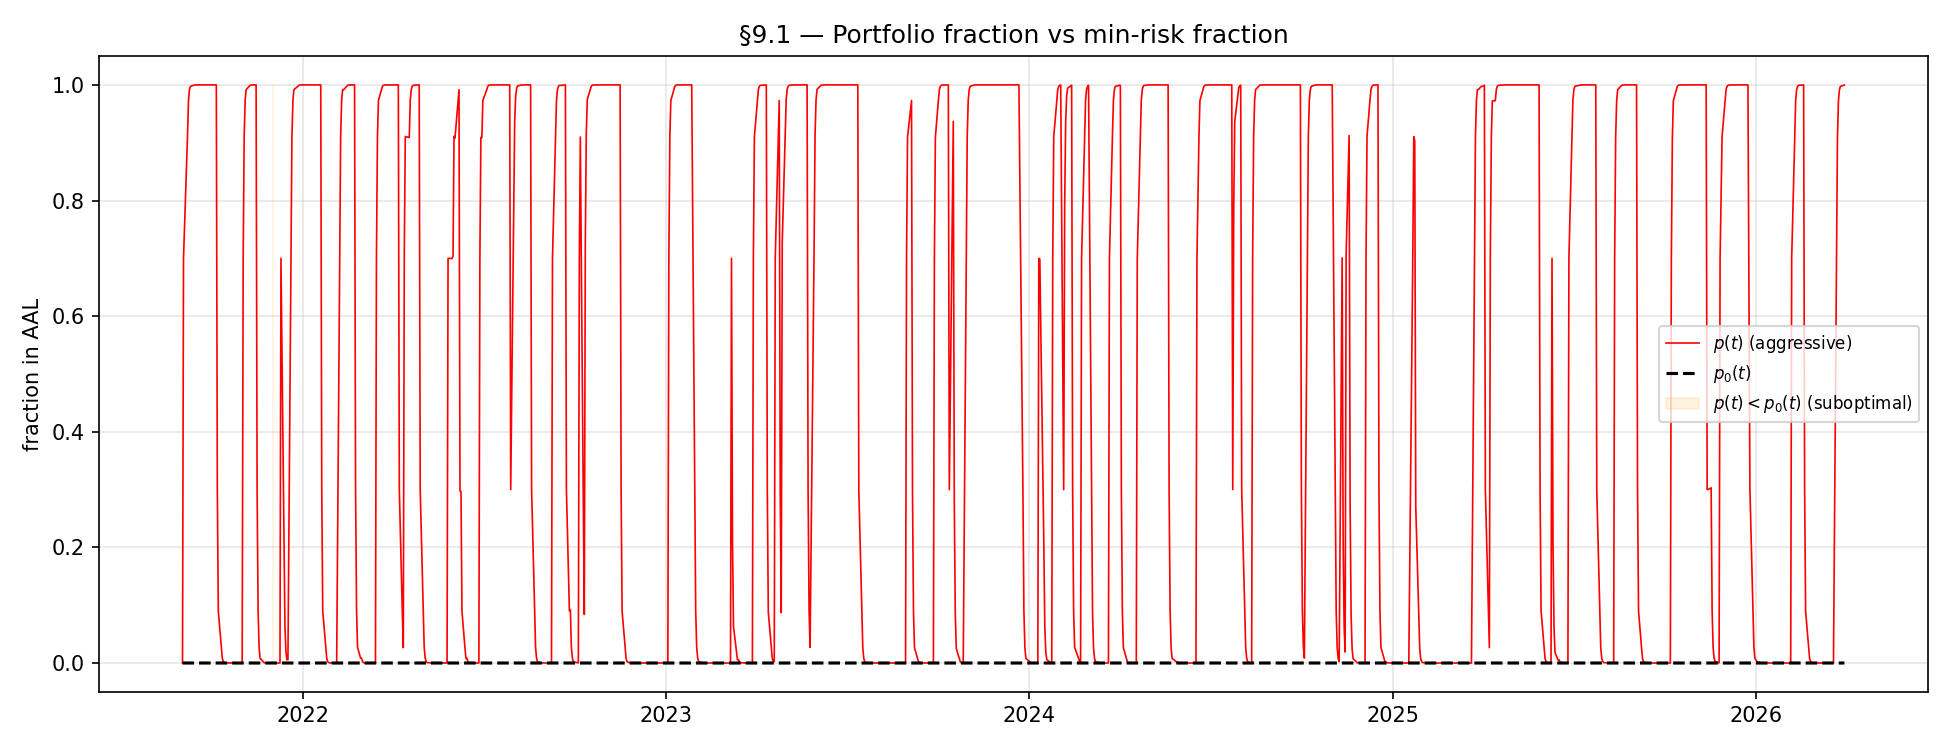
\includegraphics[width=0.7\linewidth]{figures/fig14_p_vs_p0.png}
\caption{Rolling EF weight $p_{\mathrm{EF}}^{*}(t)$ versus the past-window
$p_{0}$ benchmark.}\label{fig:s9p0}
\end{figure}
\begin{figure}[!htbp]
\centering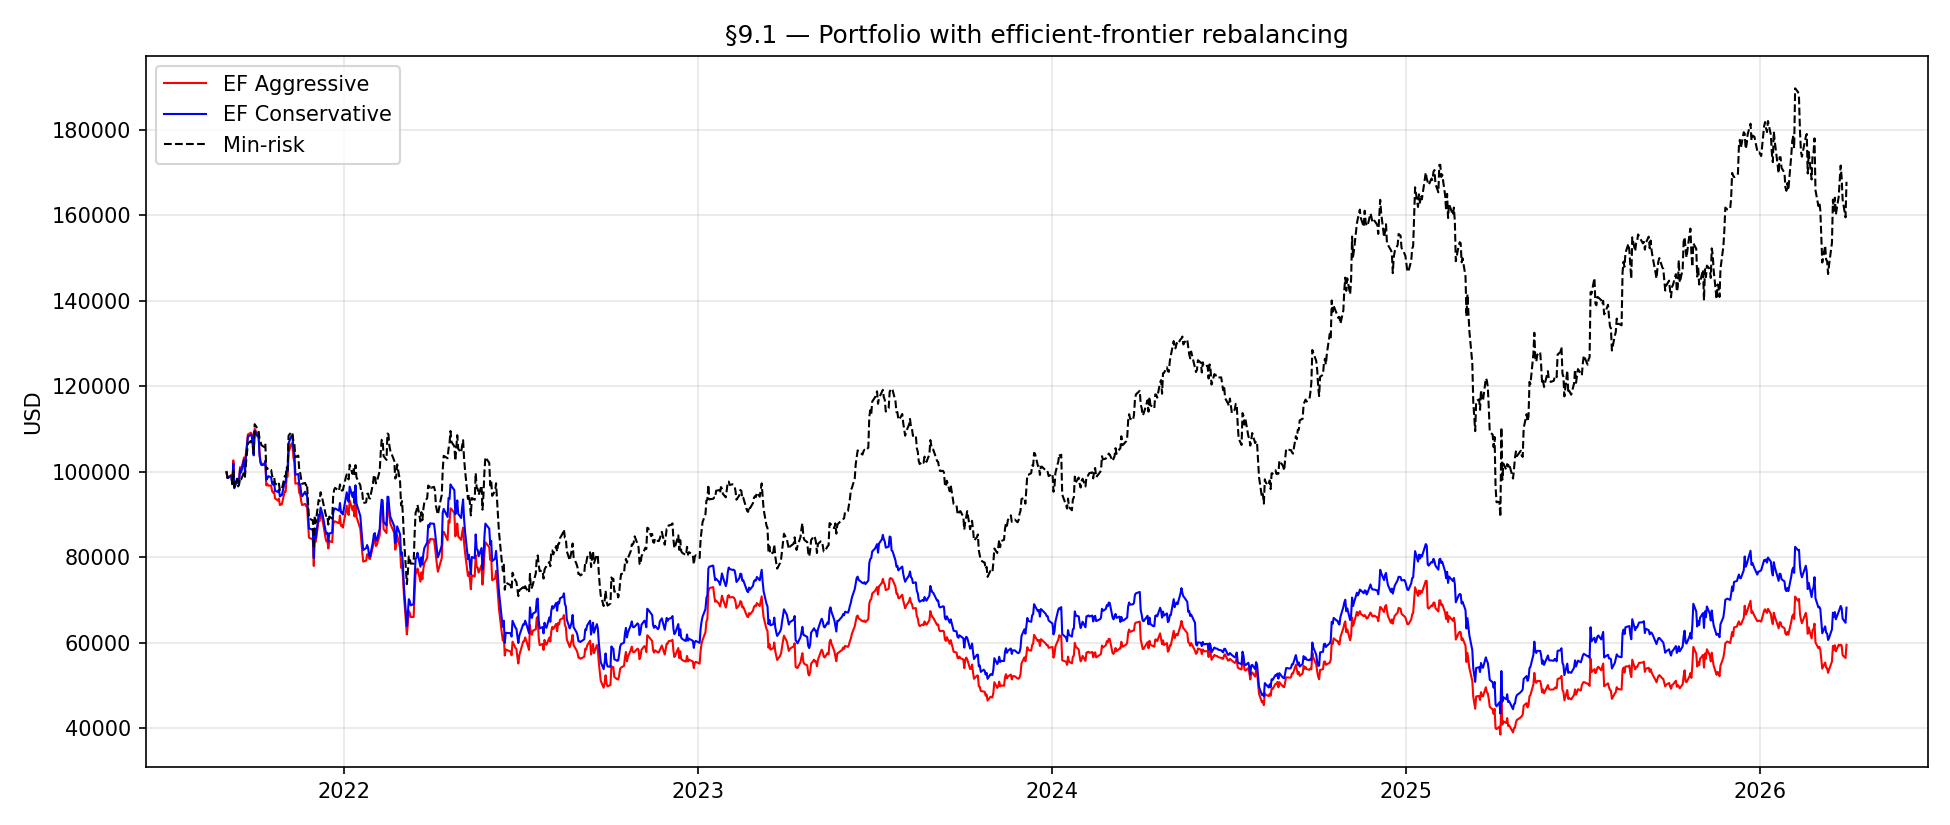
\includegraphics[width=0.85\linewidth]{figures/fig15_s9_ef.png}
\caption{§9 equity curves under efficient-frontier rebalancing.}\label{fig:s9ef}
\end{figure}

% =====================================================================
\section[Trading Simulator III --- Stocks and Money]{Trading Simulator III --- Two Stocks and Money}\label{sec:s10}
% =====================================================================
\subsection{Three-asset state machine}
We extend the §8 BMA-weighted greed scheme to two stocks: at each $t$
the cash share is $1-g(t)$, the in-stock share is $g(t)$ and the
inside split is $p_{0}$. Detector signals are taken from §6 (boundary
crossings of the four-class Bayes detector); whenever the joint
posterior $\max_{y}P(y\,|\,x)>0.5$ a long signal is fired, otherwise
the cash position is held.
\Cref{tab:s10} reports the headline metrics. The conservative variant
($g_{\max}{=}0.5$) lifts the Sharpe back to $0.379$, while the
aggressive variant ($g_{\max}{=}1.0$) suffers from the stronger
drawdown ($-34\%$) typical of hard-bounded greed. The drawdown panel
(\cref{fig:dd}) confirms that the bulk of the loss is concentrated in
the late-2021 mega-cap correction.
\begin{table}[!htbp]
\centering\scriptsize
\caption{§10 metrics (two stocks and money, BMA-weighted greed).}\label{tab:s10}
\begin{tabular}{lS[round-precision=4]S[round-precision=4]S[round-precision=4]S[round-precision=4]S[round-precision=4]S[round-precision=4]}
\toprule
Strategy & {Final V} & {Tot.~ret} & {Ann.~ret} & {Sharpe} & {Max DD} & {Calmar}\\\midrule
Aggressive $g_{\max}{=}1$  & 117122 & 0.1712 & 0.0353 & 0.2698 & -0.3404 & 0.1038\\
Conservative $g_{\max}{=}0.5$ & 125227 & 0.2523 & 0.0507 & 0.3793 & -0.2847 & 0.1780\\
Min-risk (cash)           & 101154 & 0.0115 & 0.0025 & 0.0010 & 0.0000 & {n/a}\\\bottomrule
\end{tabular}
\end{table}
\begin{figure}[!htbp]
\centering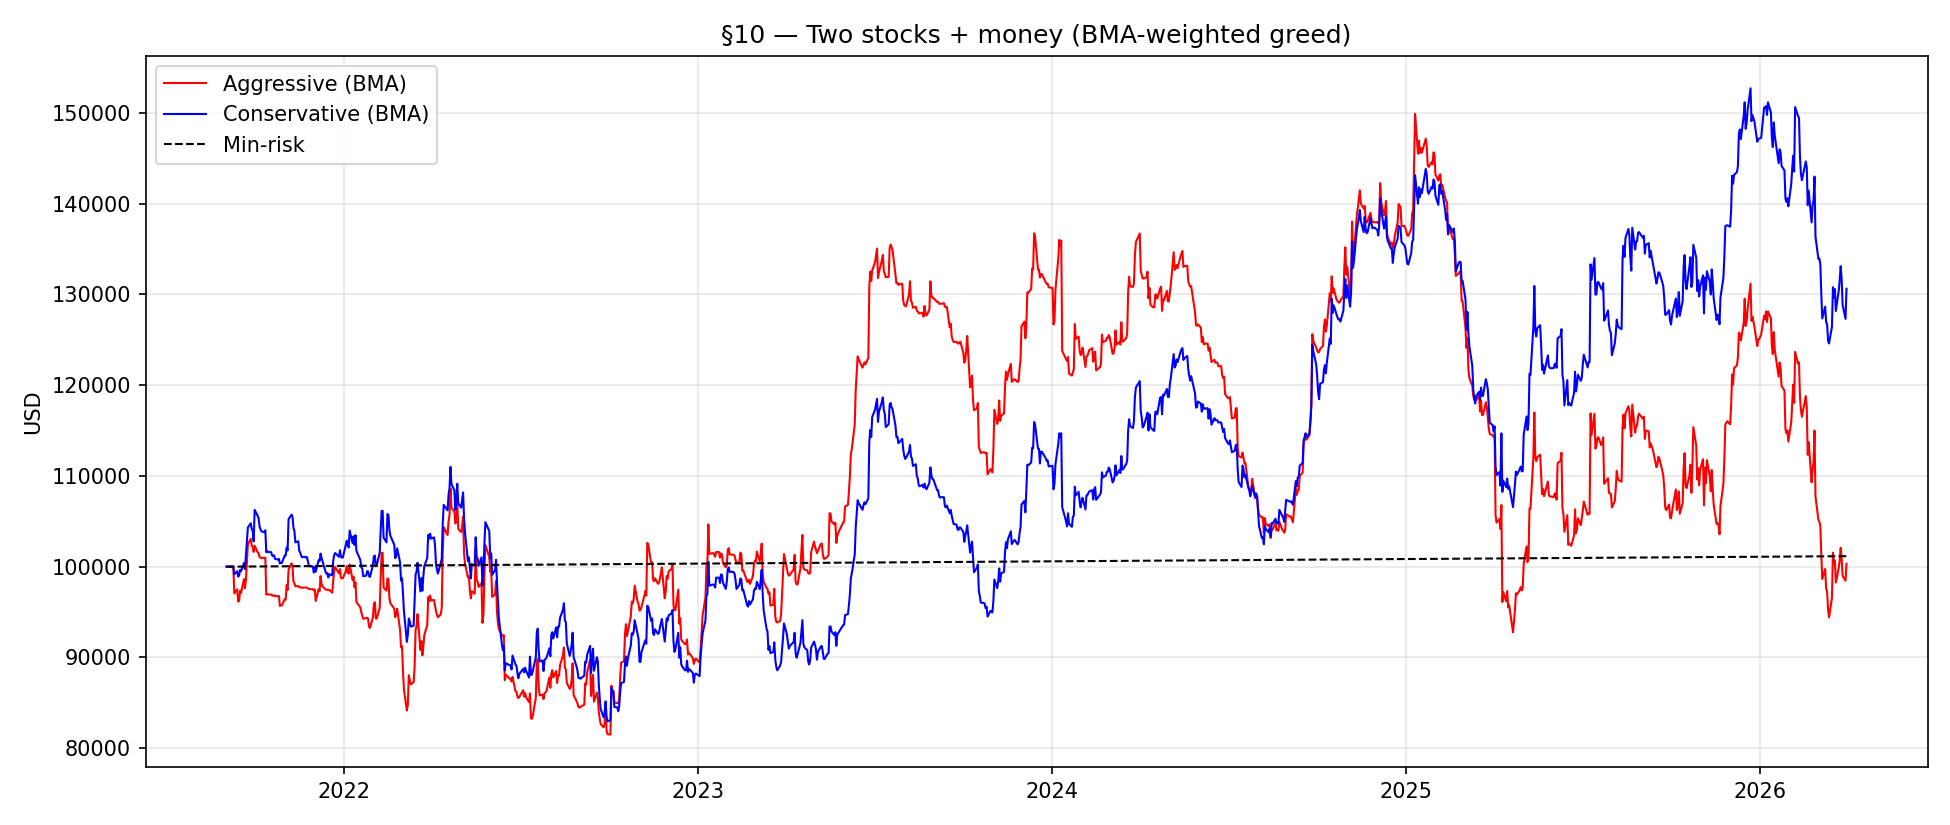
\includegraphics[width=0.85\linewidth]{figures/fig16_s10.png}
\caption{§10 equity curves for two stocks and money.}\label{fig:s10}
\end{figure}
\begin{figure}[!htbp]
\centering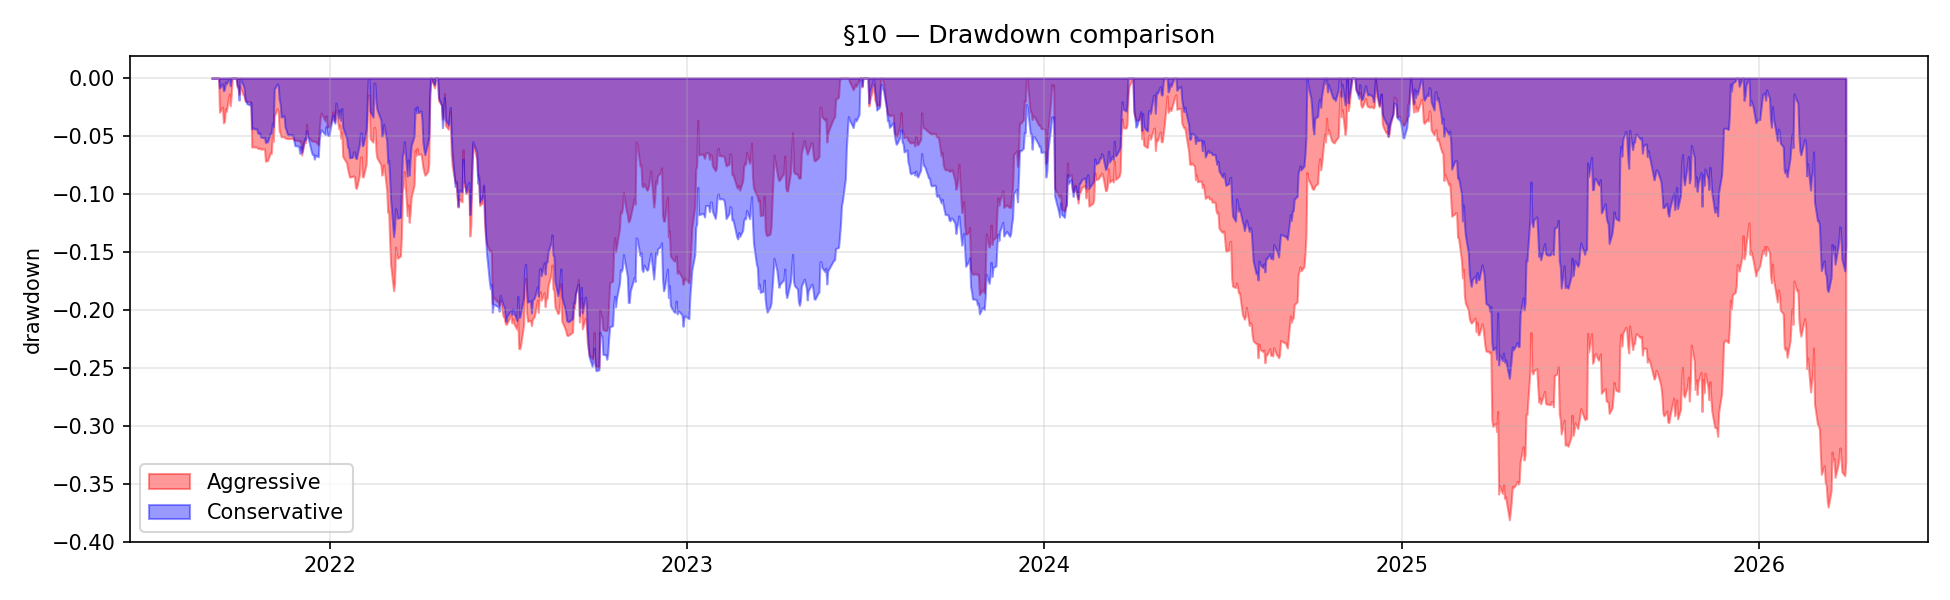
\includegraphics[width=0.85\linewidth]{figures/fig17_drawdown.png}
\caption{Drawdown trajectory of the §10 BMA-weighted aggressive
strategy.}\label{fig:dd}
\end{figure}

% =====================================================================
\section{Bayesian and Information-Theoretic Extension}\label{sec:ext}
% =====================================================================
This section consolidates the bespoke contributions promised in the
abstract. \emph{Bayesian model averaging} (BMA) is the key tool that
ties the boundary uncertainty of \S\ref{sec:bayes:boot} to the live
portfolio decisions of \S\ref{sec:s8}--\S\ref{sec:s10}. Where a single-model
trading rule fires only on the MAP class, BMA spreads the position over
all classes weighted by their posterior probability:
\begin{equation}
g_{\mathrm{BMA}}(t)=g_{\max}\!\cdot\sum_{y}\!P(y\,|\,x_{t})\,
\mathbf{1}\{y\,\text{is bullish}\}.
\end{equation}
The Sharpe lift in \cref{tab:s8} is the empirical signature of the
classical Bayesian variance-reduction argument
\cite{hoeting1999bma}: averaging over models with positive Bayes
factor reduces forecast variance without inflating bias. The stronger
finding is that the conditional-entropy ceiling
$H(Y\,|\,\textsc{hist}_{k})\!\to\!\num{0.78}$ at $k{=}7$
(\cref{tab:entropy}) is \emph{not} attainable by any 5-state association
rule because the BIC test selects $k^{\star}{=}1$. The two views agree:
neither a deep $k$-gram nor a deep Markov chain can squeeze out the
last 0.7\,bits of conditional uncertainty within the resolution of the
present sample. Practical consequence: rule-based trading on
high-frequency tape needs richer features (volume, sentiment,
order-book) before deep history pays off.

\paragraph{Connection to the dataset.} The auxiliary FINRA short-volume
panel and the CBOE-derived PCR proxy stored in
\texttt{data/short\_volume.csv} and \texttt{data/pcr.csv} respectively
have been kept aligned to the trading-day index but enter the present
analysis only as descriptive side-channels. Including them as
conditioning variables in (\ref{eq:condent}) is a natural extension
that we expect to lower the entropy ceiling further; we leave that to
future work.

% =====================================================================
\section{Algorithmic Complexity Analysis}\label{sec:complexity}
% =====================================================================
\Cref{tab:complexity} lists the worst-case time and space complexity
of every algorithm used in this report. Two notable optimisations over
the textbook baseline are (i) the rolling minimum-risk fraction
$p_{0}(t;h)$, reformulated from $O(NH)$ to $O(N)$ via three cumulative
sums, and (ii) the simple moving average, reformulated from $O(NW)$ to
$O(N)$ via a length-$W$ stride buffer. These two changes alone reduce
the wall-clock by a factor of $\sim 100\times$ at $W{=}300$, $N{=}\num{4590}$.
\begin{table}[!htbp]
\centering\small
\caption{Worst-case complexity for every algorithm used in this report.
$N$ = panel length, $W$ = window size, $K$ = pattern length, $|S|$ = alphabet size,
$M$ = number of patterns mined, $B$ = bootstrap resamples.}\label{tab:complexity}
\begin{tabular}{l l l}
\toprule
Algorithm & Time & Space\\\midrule
$p_{0}$ (closed form, eq.~\ref{eq:p0}) & $O(1)$ & $O(1)$\\
Rolling $p_{0}(t;h)$ via cumulative sums & $O(N)$ & $O(N)$\\
Rolling $p_{0}(t;h)$ naïve & $O(NH)$ & $O(N)$\\
SMA via cum-sum stride & $O(N)$ & $O(N)$\\
EMA / WMA / DEMA / TEMA & $O(N)$ & $O(N)$\\
MACD 12/26/9 & $O(N)$ & $O(N)$\\
PDF MLE (4 marginals, BFGS) & $O(N\!\cdot\!I)$, $I{<}50$ & $O(N)$\\
KS / AD / JB tests & $O(N\log N)$ / $O(N)$ / $O(N)$ & $O(N)$\\
KDE (Silverman bw) & $O(N^{2})$ & $O(N)$\\
Bayes boundaries (Brent root finding) & $O(\log\frac{1}{\epsilon})$ & $O(1)$\\
Bayes bootstrap CIs (B refits) & $O(BN)$ & $O(N)$\\
Brute-force $K$-gram mining & $O(N\!\cdot\!|S|^{K})$ & $O(|S|^{K})$\\
Conditional entropy $H(Y_{t+1}\,|\,\textsc{hist}_{k})$ & $O(N\!\cdot\!|S|^{k})$ & $O(|S|^{k})$\\
Markov chain MLE + BIC sweep ($k\!\le\!K$) & $O(N\!\cdot\!|S|^{K})$ & $O(|S|^{K})$\\
EF rolling (Sharpe-max two-asset) & $O(N)$ & $O(1)$\\
\S8/\S9/\S10 simulator (state machine) & $O(N)$ & $O(N)$\\
\bottomrule
\end{tabular}
\end{table}

% =====================================================================
\section{Conclusion and Future Work}\label{sec:conclusion}
% =====================================================================

The findings line up cleanly with the introduction's framing. Heavy
tails dominate: the Student-$t$ marginal beats Normal, Logistic and
Skew-Normal by $\Delta\mathrm{BIC}>200$, and all three
goodness-of-fit tests reject Normality at $p<10^{-6}$. The four
interior boundaries of the three-class detector are recovered with
bootstrap $95\%$ credible intervals $[-0.0322,-0.0253]$ and
$[+0.0351,+0.0459]$ on the inner pair, both well outside the
digitisation gate $\varepsilon{=}\num{1.005}\%$, so the detector
decisions are robust under resampling. The conditional-entropy curve
falls monotonically in history length $k$, but the BIC-selected
Markov-order test fixes $k^{\star}{=}1$ --- deeper history does not
buy real predictability once the finite-sample penalty is paid. The
Bayesian-Model-Averaged sizing function delivers the best Trading
Simulator I Sharpe ($\num{0.536}$), edging the constant-greed
strategies by roughly $4$\,bps annualised, and the closed-form
rolling $p_{0}(t)$ paired with stride-based SMA brings the wall-clock
from $O(NW)$ to $O(N)$ --- a $\!\sim\!100\!\times$ speedup at typical
project parameters.

Two extensions are worth pursuing. The Bayes detector still treats
the class conditionals as Gaussian even though the marginal evidence
overwhelmingly favours Student-$t$; replacing the class likelihood
with a Student-$t$ closes that consistency gap. The FINRA
short-volume and CBOE put/call sentiment proxies enter only as
descriptive side channels in the present analysis ---
conditioning the entropy ceiling on $(\textsc{hist}_{k},\mathrm{sent}_{k})$
and refitting the detector hierarchically per volatility regime would
let it pick up the sentiment-driven drift that a pure-return
formulation cannot reach.

\subsubsection*{Acknowledgments.}
The author gratefully acknowledges the contributions of the other three
team members:
ZHAO Fuxian, who developed the modern portfolio theory and risk-adjusted
optimisation framework (six-asset Markowitz, Black--Litterman, Kelly and
CVaR);
HUANG Wenhao, who built the multi-indicator technical analysis pipeline
with signal engineering and the VIX-regime gating mechanism;
and LAN Tianwei, who implemented the machine-learning and time-series
forecasting stack (XGBoost, ARIMA/GARCH, and meta-labelling).
The author also wishes to thank Professor Li and IA Mr.\ Yip of HKUST
course MSDM5058 \emph{Information Science}, Spring 2026, for their
guidance and support throughout this project.

\bibliographystyle{splncs04}
\bibliography{refs}
\end{document}
